% notes
\providecommand{\redo}[1]{{\color{red} #1}}
\providecommand{\rebuttal}[1]{{#1}}


\providecommand{\nbc}[3]{
 {\colorbox{#3}{\bfseries\sffamily\scriptsize\textcolor{white}{#1}}}
 {\textcolor{#3}{\sf\small\textit{#2}}}
 }
\definecolor{annotcolo}{rgb}{0.1,0.1,0.9}
\providecommand{\nj}[1]{\nbc{NJ}{#1}{annotcolo}}


% config
\providecommand{\smalltextsc}[1]{\textsc{\small #1}}
\providecommand{\scripttextsc}[1]{\textsc{\scriptsize #1}}
\providecommand{\tinytextsc}[1]{\textsc{\tiny #1}}

% sysnames
\providecommand{\livecodebench}{\smalltextsc{LiveCodeBench}}
\providecommand{\lcb}{\smalltextsc{LCB}}
\providecommand{\livecodebenchtitle}{\textsc{LiveCodeBench}}


% general
\providecommand{\llm}{\smalltextsc{LLM}\xspace}
\providecommand{\llms}{\smalltextsc{LLMs}\xspace}
\providecommand{\chainot}{\smalltextsc{COT}\xspace}
\providecommand{\python}{\smalltextsc{Python}\xspace}




%models

%openai
\providecommand{\openai}{\smalltextsc{OpenAI}}
\providecommand{\gpts}{\smalltextsc{GPTs}\xspace}
\providecommand{\codedavinci}{\smalltextsc{Code-Davinci-002}\xspace}
\providecommand{\gptthreefiveturbo}{\smalltextsc{GPT-3.5-turbo}\xspace}
\providecommand{\gptfour}{\smalltextsc{GPT-4}\xspace}
\providecommand{\gptfourturbo}{\smalltextsc{GPT-4-Turbo}\xspace}
\providecommand{\gptfouro}{\smalltextsc{GPT-4-O}\xspace}

%deepmind
\providecommand{\alphacode}{\smalltextsc{AlphaCode}\xspace}
\providecommand{\alphacodeB}[1]{\smalltextsc{AlphaCode-#1B}\xspace}

%anthropic
\providecommand{\claude}{\smalltextsc{Claude}\xspace}
\providecommand{\claudes}{\smalltextsc{Claudes}\xspace}
\providecommand{\claudetwo}{\smalltextsc{Claude-2}\xspace}
\providecommand{\claudethrees}{\smalltextsc{Claude-3s}\xspace}
\providecommand{\claudeinstantone}{\smalltextsc{Claude-Ins-1}\xspace}
\providecommand{\claudeopus}{\smalltextsc{Claude-3-Opus}\xspace}
\providecommand{\claudesonnet}{\smalltextsc{Claude-3-Sonnet}\xspace}

%google
\providecommand{\gemini}{\smalltextsc{Gemini}\xspace}
\providecommand{\geminis}{\smalltextsc{Geminis}\xspace}
\providecommand{\geminipro}{\smalltextsc{Gemini-Pro}\xspace}
\providecommand{\geminiproonefive}{\smalltextsc{Gemini-Pro-1.5}\xspace}
\providecommand{\geminiflash}{\smalltextsc{Gemini-Flash}\xspace}
\providecommand{\geminiultra}{\smalltextsc{Gemini-Ultra}\xspace}

%meta 
\providecommand{\cllamas}{\smalltextsc{CodeLLaMas}\xspace}
\providecommand{\cllama}{\smalltextsc{CodeLLaMa}\xspace}
\providecommand{\cllamains}{\smalltextsc{CodeLLaMa-Ins}\xspace}
\providecommand{\cllamabase}{\smalltextsc{CodeLLaMa-Base}\xspace}
\providecommand{\cllamaB}[1]{\smalltextsc{CL-Ins-#1B}\xspace}
\providecommand{\cllamacommonB}[1]{CL-#1B}
\providecommand{\cllamabaseB}[1]{\smalltextsc{CL-Base-#1B}\xspace}
\providecommand{\cllamaBList}{\smalltextsc{CL-Ins-\{7, 13, 34\}B}\xspace}
\providecommand{\cllamabaseBList}{\smalltextsc{CL-Base-\{7, 13, 34\}B}\xspace}

\providecommand{\llamas}{\smalltextsc{LLaMa-3s}\xspace}

\providecommand{\llamabase}{\smalltextsc{L3-Base}}
\providecommand{\llamabaselist}{\smalltextsc{L3-Base-\{7, 70\}B}\xspace}
\providecommand{\llamainslist}{\smalltextsc{L3-Ins-\{7, 70\}B}\xspace}
\providecommand{\llamaB}[1]{\smalltextsc{L3-Ins-#1B}\xspace}
\providecommand{\llamabaseB}[1]{\smalltextsc{L3-Base-#1B}\xspace}

%finetunes
\providecommand{\wizardlong}{\smalltextsc{WizardCoder}\xspace}
\providecommand{\wizard}{\smalltextsc{WC-34B}\xspace}
\providecommand{\wizardtwo}{\smalltextsc{WC-33B}\xspace}
\providecommand{\phind}{\smalltextsc{Phind-34B}\xspace}
\providecommand{\magicoders}{\smalltextsc{MagiCoders}\xspace}
\providecommand{\magicoder}[1]{\smalltextsc{MC-#1B}\xspace}
\providecommand{\magicoderBLit}{\smalltextsc{MC-\{6.7, 7\}B}\xspace}

%deepseek
\providecommand{\deepseek}{\smalltextsc{DeepSeek}\xspace}
\providecommand{\deepseekbase}{\smalltextsc{DeepSeek-Base}\xspace}
\providecommand{\deepseekinstruct}{\smalltextsc{DeepSeek-Instruct}\xspace}
\providecommand{\deepseeks}{\smalltextsc{DeepSeeks}\xspace}
\providecommand{\deepseekcode}[1]{\smalltextsc{DS}-#1B\xspace}
\providecommand{\deepseekcodeins}{\smalltextsc{DS-Ins}\xspace}
\providecommand{\deepseekcodeB}[1]{\smalltextsc{DS-Ins-#1B}\xspace}
\providecommand{\deepseekbaseB}[1]{\smalltextsc{DS-Base-#1B}\xspace}
\providecommand{\deepseekcodeBList}{\smalltextsc{DS-Ins-\{1.3, 6.7, 33\}B}\xspace}
\providecommand{\deepseekcodebaseBList}{\smalltextsc{DS-Base-\{1.3, 6.7, 33\}B}\xspace}

% codeqwen
\providecommand{\codeqwen}{\smalltextsc{CodeQwen}\xspace}
\providecommand{\codeqwenchat}{\smalltextsc{CodeQwen-Chat}\xspace}

%mistral

\providecommand{\mixtral}{\smalltextsc{Mixtral}\xspace}
\providecommand{\codestral}{\smalltextsc{Codestral}\xspace}
\providecommand{\mistrallarge}{\smalltextsc{Mistral-L}\xspace}
\providecommand{\mistral}{\smalltextsc{Mistral}\xspace}

% bigcode

\providecommand{\starcoder}{\smalltextsc{StarCoder}\xspace}
\providecommand{\starcodertwo}{\smalltextsc{StarCoder2}\xspace}
\providecommand{\starcodertwobase}{\smalltextsc{StarCoder2-Base}\xspace}
\providecommand{\sctwoinsB}[1]{\smalltextsc{SC2-#1B}\xspace}
\providecommand{\sctwobaseB}[1]{\smalltextsc{SC2-Base-#1B}\xspace}
\providecommand{\sctwobaseBList}{\smalltextsc{SC2-Base-\{3,7,15\}B}\xspace}

% cohere
\providecommand{\commandr}{\smalltextsc{CMD-R}\xspace}
\providecommand{\commandrplus}{\smalltextsc{CMD-R+}\xspace}


% datasets
\providecommand{\thestack}{\smalltextsc{Stack}\xspace}
\providecommand{\apps}{\smalltextsc{APPS}\xspace}
\providecommand{\contests}{\smalltextsc{Code-Contests}\xspace}
\providecommand{\humaneval}{\smalltextsc{HumanEval}}
\providecommand{\humanevalplus}{\smalltextsc{HumanEval+}}
\providecommand{\mbpp}{\smalltextsc{MBPP}}
\providecommand{\cruxeval}{\smalltextsc{CRUXEval}}
\providecommand{\codet}{\smalltextsc{CodeT}}
\providecommand{\xcode}{\smalltextsc{xCodeEval}\xspace}
\providecommand{\codescope}{\smalltextsc{CodeScope}\xspace}
\providecommand{\taco}{\smalltextsc{TACO}\xspace}
\providecommand{\usacobench}{\smalltextsc{USCAOBench}\xspace}
%coding websites
\providecommand{\leetcode}{\smalltextsc{LeetCode}\xspace}
\providecommand{\atcoder}{\smalltextsc{AtCoder}\xspace}
\providecommand{\codeforces}{\smalltextsc{CodeForces}\xspace}
\providecommand{\html}{\smalltextsc{HTML}\xspace}

\providecommand{\easy}{\smalltextsc{Easy}\xspace}
\providecommand{\medium}{\smalltextsc{Medium}\xspace}
\providecommand{\hard}{\smalltextsc{Hard}\xspace}

%website scrapes
\providecommand{\problem}{\smalltextsc{$P$}\xspace}
\providecommand{\solution}{\smalltextsc{$S$}\xspace}
\providecommand{\tests}{\smalltextsc{$T$}\xspace}
\providecommand{\testspublic}{\smalltextsc{$T_{p}$}\xspace}
\providecommand{\testshidden}{\smalltextsc{$T_{h}$}\xspace}
\providecommand{\contestdate}{\smalltextsc{$D$}\xspace}

% metrics
\providecommand{\passmetric}[1]{\smalltextsc{Pass@}#1\xspace}



% %%%%
\lstset{
  basicstyle=\ttfamily\small,
  columns=fullflexible,
  % frame=single,
  breaklines=true,
  postbreak=\mbox{$\hookrightarrow$\space},
  rulecolor=\color{black},
}
\definecolor{codegreen}{rgb}{0,0.6,0}
\lstdefinestyle{mystyle}{  
    commentstyle=\color{codegreen},
    keywordstyle=\color{blue},
    basicstyle=\ttfamily\small,
    breakatwhitespace=false,        
    breaklines=true,                 
    captionpos=b,                    
    keepspaces=true,                 
    showspaces=false,                
    showstringspaces=false,
    showtabs=false,                  
    tabsize=2
}
\lstset{style=mystyle}

% if you use cleveref..

% %%%%%%%%%%%%%%%%%%%%%%%%%%%%%%%%
% % THEOREMS
% %%%%%%%%%%%%%%%%%%%%%%%%%%%%%%%%
% \theoremstyle{plain}
% \newtheorem{theorem}{Theorem}[section]
% \newtheorem{proposition}[theorem]{Proposition}
% \newtheorem{lemma}[theorem]{Lemma}
% \newtheorem{corollary}[theorem]{Corollary}
% \theoremstyle{definition}
% \newtheorem{definition}[theorem]{Definition}
% \newtheorem{assumption}[theorem]{Assumption}
% \theoremstyle{remark}
% \newtheorem{remark}[theorem]{Remark}

% % Todonotes is useful during development; simply uncomment the next line
% %    and comment out the line below the next line to turn off comments

% \input{math_commands.tex}
% \newcommand{\todo}[1]{\textcolor{red}{[TODO: #1]}}
\newcommand{\term}[1]{\emph{#1}}
\definecolor{rewriteblue}{RGB}{0,70,170}
\definecolor{mygreen}{RGB}{226,240,217}
\definecolor{myblue}{RGB}{222,235,247}
\definecolor{myorange}{RGB}{251,229,214}
\definecolor{lightblue}{RGB}{232,242,255}
\definecolor{lightorange}{RGB}{255,241,224}
\definecolor{good}{HTML}{1B7837}
\definecolor{bad}{HTML}{B2182B}
\newcommand{\needsrewrite}[1]{\textcolor{rewriteblue}{[SOURCE-DERIVED; REWRITE: #1]}}
\newenvironment{rewriteblock}{%
  \par\begingroup\color{rewriteblue}%
  \noindent
}{%
  \par\endgroup
}
\newenvironment{draftblock}{%
  \par\noindent
}{%
  \par
}
\newcommand{\sourcepaper}[2]{}

\definecolor{lightgreen}{HTML}{C4FFCF}
\definecolor{codegreen}{rgb}{0,0.6,0}

\newcommand{\red}[1]{\textbf{\textcolor{red}{#1}}}
\newcommand{\green}[1]{\textbf{\textcolor{ForestGreen}{#1}}}
\newcommand{\cmark}{\ding{51}}
\newcommand{\xmark}{\ding{55}}
\newcommand{\benchmark}{\textsc{CRUXEval}\xspace}
\newcommand{\benchmarki}{\textsc{CRUXEval-I}\xspace}
\newcommand{\benchmarko}{\textsc{CRUXEval-O}\xspace}
\newcommand{\codellamamed}{\textsc{Code Llama 13B}\xspace}
\newcommand{\codellamalarge}{\textsc{Code Llama 34B}\xspace}
\providecommand{\multirow}[3]{#3}
\providecommand{\hdashline}[1][]{\midrule}
\NewDocumentCommand{\cdashline}{m o}{}
\providecommand{\makecell}[1]{\begin{tabular}{@{}c@{}}#1\end{tabular}}
\providecommand{\smallsec}[1]{\textbf{#1\,\,}}
\providecommand{\llm}{\textsc{LLM}\xspace}
\providecommand{\llms}{\textsc{LLMs}\xspace}
\providecommand{\lean}{\textsc{Lean}\xspace}
\providecommand{\setstretch}[1]{}
\providecommand{\smallsim}{\mathrel{\sim}}
\providecommand{\subfloat}[2][]{%
  \begin{minipage}{0.49\textwidth}%
  \centering
  #2%
  \if\relax\detokenize{#1}\relax\else\subcaption{#1}\fi
  \end{minipage}%
}

\DeclareMathOperator*{\argmax}{arg\,max}
\DeclareMathOperator*{\argmin}{arg\,min}
\lstdefinelanguage{Lean}{
  morekeywords={theorem,lemma,def,by,have,show,calc,let,fun,match,with,if,then,else,import,open,namespace,end,where,structure,inductive,example},
  sensitive=true,
  morecomment=[l]{--},
  morecomment=[s]{/-}{-/},
  morestring=[b]"
}
\lstdefinelanguage{triton}{
  morekeywords={tl,triton,jit,program_id,load,store,arange,zeros,where,constexpr,block_ptr,dtype},
  sensitive=true,
  morecomment=[l]{\#},
  morestring=[b]"
}
\lstdefinelanguage{CUDA}{
  morekeywords={__global__,__device__,__shared__,__constant__,__host__,__syncthreads,threadIdx,blockIdx,blockDim,gridDim},
  sensitive=true,
  morecomment=[l]{//},
  morecomment=[s]{/*}{*/},
  morestring=[b]",
  morestring=[b]'
}
\lstdefinelanguage{Rust}{
  morekeywords={as,break,const,continue,crate,else,enum,extern,false,fn,for,if,impl,in,let,loop,match,mod,move,mut,pub,ref,return,self,Self,static,struct,super,trait,true,type,unsafe,use,where,while,async,await,dyn},
  sensitive=true,
  morecomment=[l]{//},
  morecomment=[s]{/*}{*/},
  morestring=[b]",
  morestring=[b]'
}
\lstdefinelanguage{Python}{
  morekeywords={and,as,assert,break,class,continue,def,del,elif,else,except,False,finally,for,from,global,if,import,in,is,lambda,None,nonlocal,not,or,pass,raise,return,True,try,while,with,yield},
  sensitive=true,
  morecomment=[l]{\#},
  morecomment=[s]{\"\"\"}{\"\"\"},
  morecomment=[s]{\'\'\'}{\'\'\'},
  morestring=[b]',
  morestring=[b]"
}
\lstdefinelanguage{json}{
  morekeywords={true,false,null},
  sensitive=false,
  morestring=[b]",
  morecomment=[l]{//},
}

\lstdefinestyle{mystyle}{
  commentstyle=\color{codegreen},
  keywordstyle=\color{blue},
  basicstyle=\ttfamily\footnotesize,
  breakatwhitespace=false,
  breaklines=true,
  captionpos=b,
  keepspaces=true,
  showspaces=false,
  showstringspaces=false,
  showtabs=false,
  tabsize=2
}
\lstdefinestyle{boxed}{
  frame=single,
  breaklines=true,
  postbreak=\mbox{$\hookrightarrow$\space},
  commentstyle=\color{codegreen},
  keywordstyle=\color{blue},
  basicstyle=\ttfamily\footnotesize,
  breakatwhitespace=false,
  captionpos=t,
  keepspaces=true,
  showspaces=false,
  showstringspaces=false,
  showtabs=false,
  tabsize=2
}
\lstdefinestyle{specblock}{
  frame=single,
  breaklines=true,
  basicstyle=\ttfamily\scriptsize,
  keepspaces=true,
  showstringspaces=false,
  columns=fullflexible
}
\DefineVerbatimEnvironment{codebox}{Verbatim}{fontsize=\small}
\DefineVerbatimEnvironment{examplecodebox}{Verbatim}{fontsize=\small}
\lstdefinestyle{reasoning}{
  breaklines=true,
  commentstyle=\color{codegreen},
  keywordstyle=\color{blue},
  breakautoindent=0pt,
  breakindent=0pt,
  basicstyle=\itshape\footnotesize,
  breakatwhitespace=true,
  captionpos=t,
  keepspaces=true,
  showspaces=false,
  showstringspaces=false,
  showtabs=false
}
\lstdefinestyle{mystylesmaller}{
  commentstyle=\color{codegreen},
  keywordstyle=\color{blue},
  basicstyle=\ttfamily\scriptsize,
  breaklines=true,
  captionpos=b,
  keepspaces=true,
  showspaces=false,
  showstringspaces=false,
  showtabs=false,
  tabsize=2
}
\lstdefinestyle{mystyletiny}{
  commentstyle=\color{codegreen},
  keywordstyle=\color{blue},
  basicstyle=\ttfamily\tiny,
  breaklines=true,
  captionpos=b,
  keepspaces=true,
  showspaces=false,
  showstringspaces=false,
  showtabs=false,
  tabsize=2
}
\lstdefinestyle{leancompact}{
  language=Lean,
  basicstyle=\fontsize{3}{3.5}\ttfamily,
  breaklines=true,
  captionpos=b,
  keepspaces=true,
  showspaces=false,
  showstringspaces=false,
  showtabs=false,
  frame=none
}
\lstset{
  style=mystyle,
  columns=fullflexible,
  frame=single,
  postbreak=\mbox{$\hookrightarrow$\space},
  rulecolor=\color{black},
  moredelim=[is][\color{red}]{!*}{*!},
  literate={₀}{{$_0$}}1
           {₁}{{$_1$}}1
           {₂}{{$_2$}}1
           {₃}{{$_3$}}1
           {₄}{{$_4$}}1
           {₅}{{$_5$}}1
           {₆}{{$_6$}}1
           {₇}{{$_7$}}1
           {₈}{{$_8$}}1
           {₉}{{$_9$}}1
           {¹}{{$^1$}}1
           {²}{{$^2$}}1
           {³}{{$^3$}}1
           {⁻}{{$^-$}}1
           {·}{{$\cdot$}}1
           {×}{{$\times$}}1
           {∀}{{$\forall$}}1
           {∃}{{$\exists$}}1
           {ℕ}{{$\mathbb{N}$}}1
           {ℚ}{{$\mathbb{Q}$}}1
           {ℝ}{{$\mathbb{R}$}}1
           {ℤ}{{$\mathbb{Z}$}}1
           {∧}{{$\wedge$}}1
           {∨}{{$\vee$}}1
           {∈}{{$\in$}}1
           {∉}{{$\notin$}}1
           {∑}{{$\sum$}}1
           {∫}{{$\int$}}1
           {∣}{{$\mid$}}1
           {≠}{{$\ne$}}1
           {≡}{{$\equiv$}}1
           {≤}{{$\le$}}1
           {≥}{{$\ge$}}1
           {←}{{$\leftarrow$}}1
           {→}{{$\to$}}1
           {↑}{{$\uparrow$}}1
           {⊢}{{$\vdash$}}1
           {⟨}{{$\langle$}}1
           {⟩}{{$\rangle$}}1
           {…}{{\ldots}}1
}

\makeatletter
\def\@captype{lstlisting}
\lst@AddToHook{Init}{\def\@captype{lstlisting}}
\makeatother

\theoremstyle{plain}
\newtheorem{theorem}{Theorem}[chapter]
\newtheorem{lemma}[theorem]{Lemma}
\newtheorem{proposition}[theorem]{Proposition}
\newtheorem{corollary}[theorem]{Corollary}

\theoremstyle{definition}
\newtheorem{definition}[theorem]{Definition}
\newtheorem{example}[theorem]{Example}

\theoremstyle{remark}
\newtheorem{remark}[theorem]{Remark}



\providecommand{\smallsim}{\smallsym{\mathrel}{\sim}}

\makeatletter
\providecommand{\smallsym}[2]{#1{\mathpalette\make@small@sym{#2}}}
\providecommand{\make@small@sym}[2]{%
  \vcenter{\hbox{$\m@th\downgrade@style#1#2$}}%
}
\providecommand{\downgrade@style}[1]{%
  \ifx#1\displaystyle\scriptstyle\else
    \ifx#1\textstyle\scriptstyle\else
      \scriptscriptstyle
  \fi\fi
}
\makeatother


In \livecodebench{}, we address two problems that made existing code benchmarks
increasingly unreliable as code models improved. The first problem is
contamination. Benchmarks such as \humaneval{}, \mbpp{}, and \apps{} are
static: once their problems are public, later models may see them during training.
Therefore, data contamination and programming ability can easily be conflated in model evaluation.

The second problem is that these coding benchmarks only measure natural language
to code generation. While this task is important, it is only one of many capabilities
that programming agents need to exhibit. Coding workflows involve repairing failed solutions,
reasoning about the execution of programs, and constructing input-output pairs for testing. To address these two gaps, \livecodebench{} combines a live, time-indexed benchmark
with a holistic multi-scenario design.

\subsection{Benchmark Construction}
\livecodebench{} continuously collects contest problems from \leetcode{},
\atcoder{}, and \codeforces{}. These platforms periodically release problems
with natural-language statements, example input-output pairs, hidden tests, and
public contest dates. \livecodebench{} records the contest date for each
problem, which makes the release date part of the benchmark instance rather
than external metadata. Therefore, we can scroll over different time windows by filtering problems
between any pair of dates.

The benchmark also emphasizes problem and test quality. Existing competitive
programming benchmarks can include problems that are difficult to evaluate by
standard input-output auto-grading, such as problems that permit multiple
correct outputs for a single input. Such problems can incorrectly penalize
valid solutions. Other benchmarks can contain insufficient tests, adding noise
to reported pass rates. \livecodebench{} uses automated scrapers and filtering
heuristics to collect problem statements, tests, ground-truth solutions, and
metadata, while excluding problems that are not suitable for reliable
input-output evaluation.

Test collection is also an important aspect of the benchmark construction across all
four scenarios. When tests are natively available through the platform, \livecodebench{}
uses them directly. Otherwise, it uses a language model to synthesize test
input generators rather than directly generating individual inputs. In addition, it
includes adversarial or stress tests where possible. 

\subsection{Effects of Contamination}
\label{subsec:livecodebench-contamination}
\noindent \textbf{Contamination in \deepseek{} and \gptfouro{}.}
\livecodebench{} curates problems released since May $2023$.
However, \deepseek{} was released Sep $2023$ and \gptfouro{}'s official cutoff date is Nov $2023$.
In Figure~\ref{fig:lcb-contamination-all-tasks-thesis}, we show the performance of these models on \leetcode{} problems released in different months from May $2023$ and Aug $2024$.
First, we notice significant drops in model performance: \deepseekcodeB{33} after Aug. $2023$ and \gptfouro{} after Nov. $2023$.
These drops align with the release/cutoff dates of the models, suggesting
that earlier problems may indeed be contaminated. 
This trend is consistent across other \livecodebench{} scenarios like repair and code execution.
We note that this performance drop occurs primarily for \leetcode{} problems, while model performance is relatively smooth across the months for problems from other platforms (Figure~\ref{fig:lcb-atcoder-contamination-thesis}),
which may suggest different levels of contamination across different sources. 

\begin{figure}[H]
    \centering
    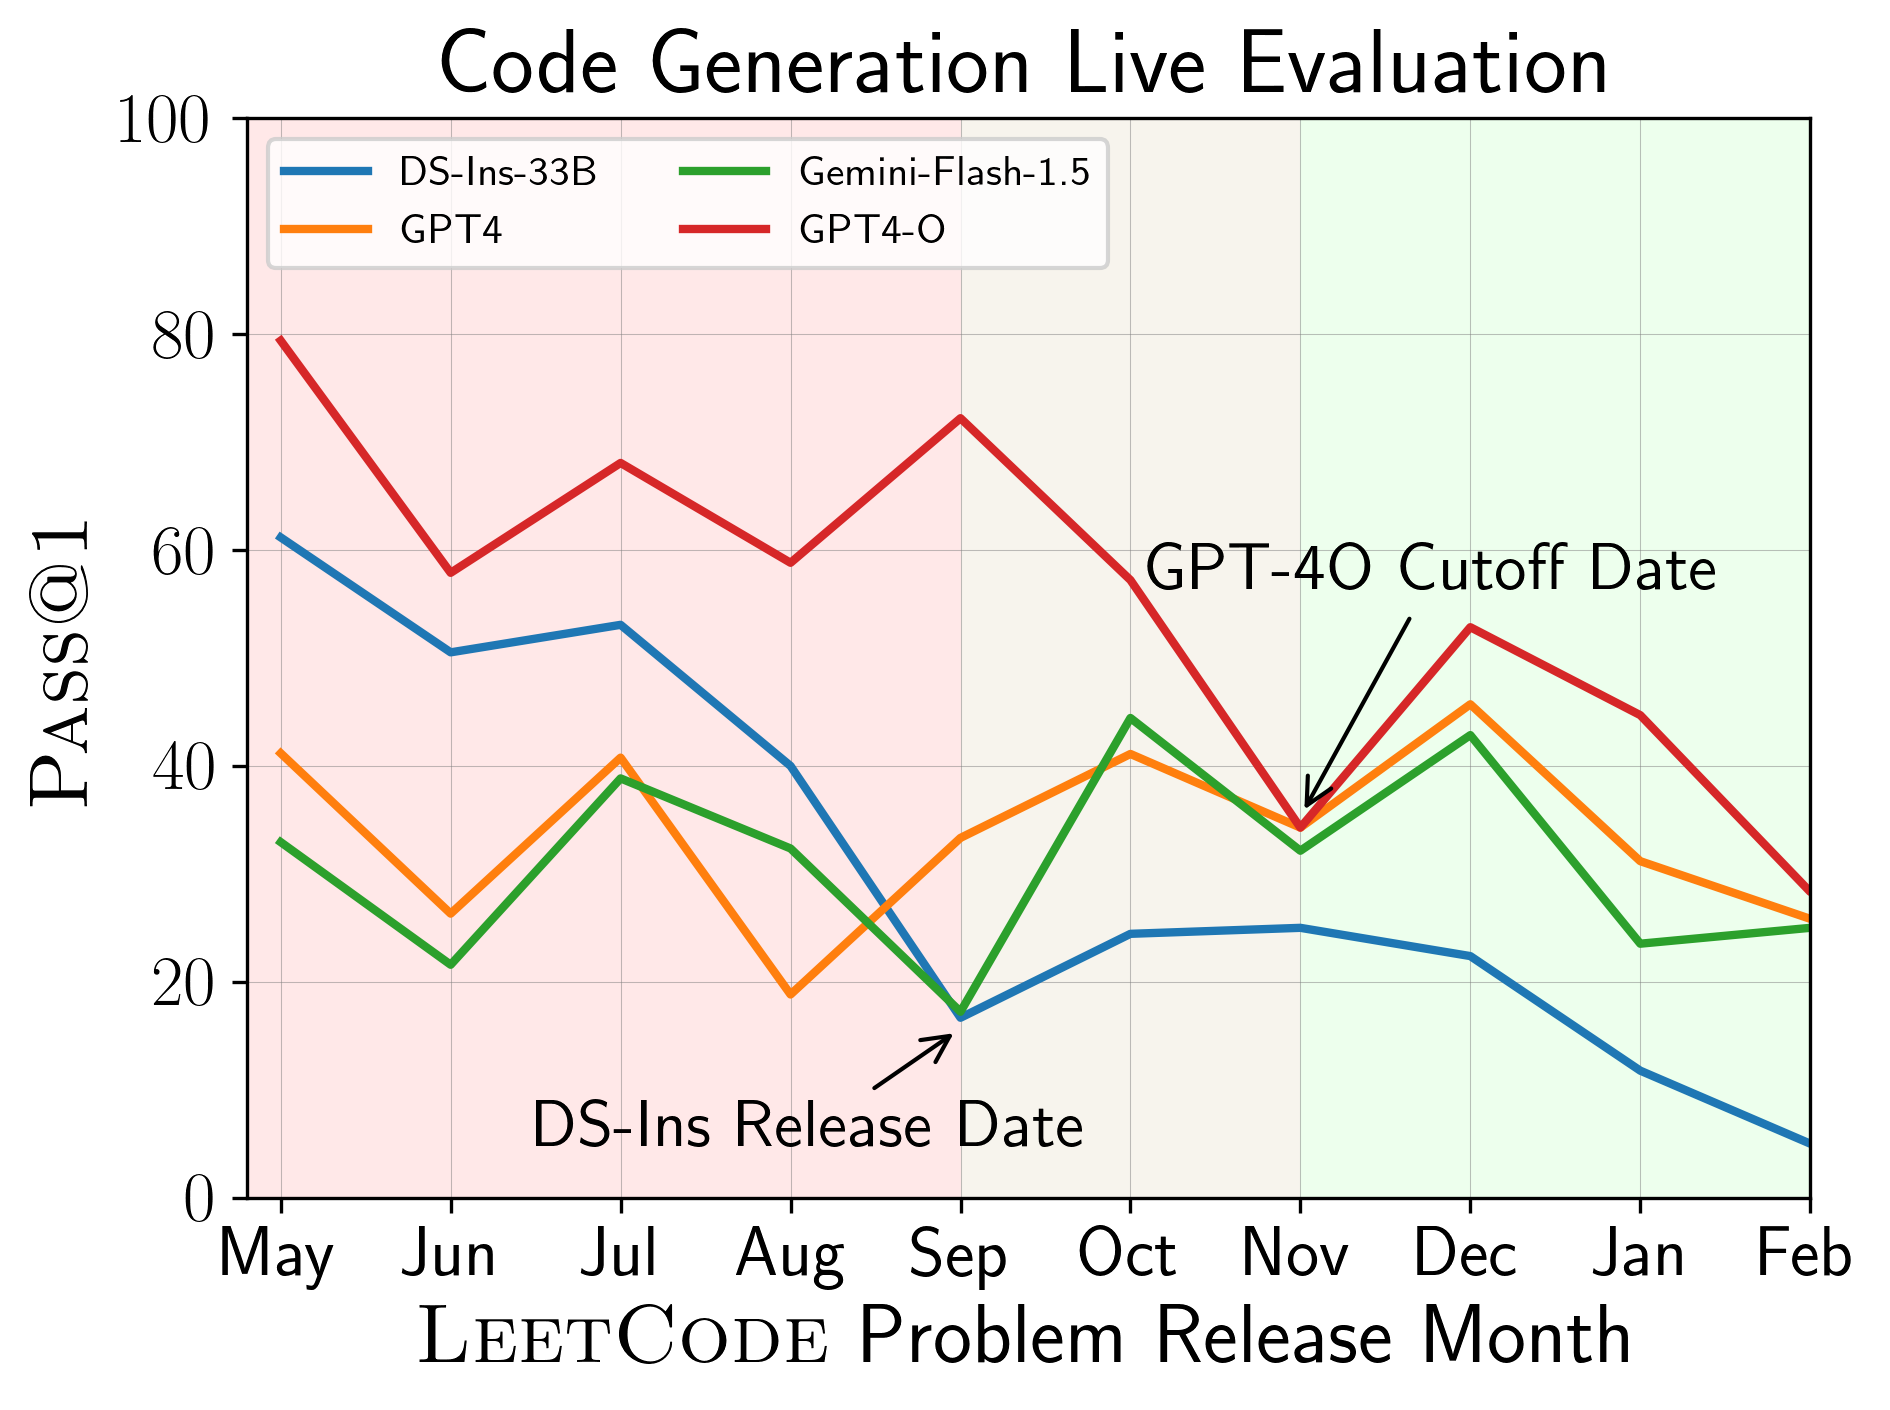
\includegraphics[width=0.49\linewidth]{figures/contamination_new/main_14_codegen_leetcode.png}
    \hfil
    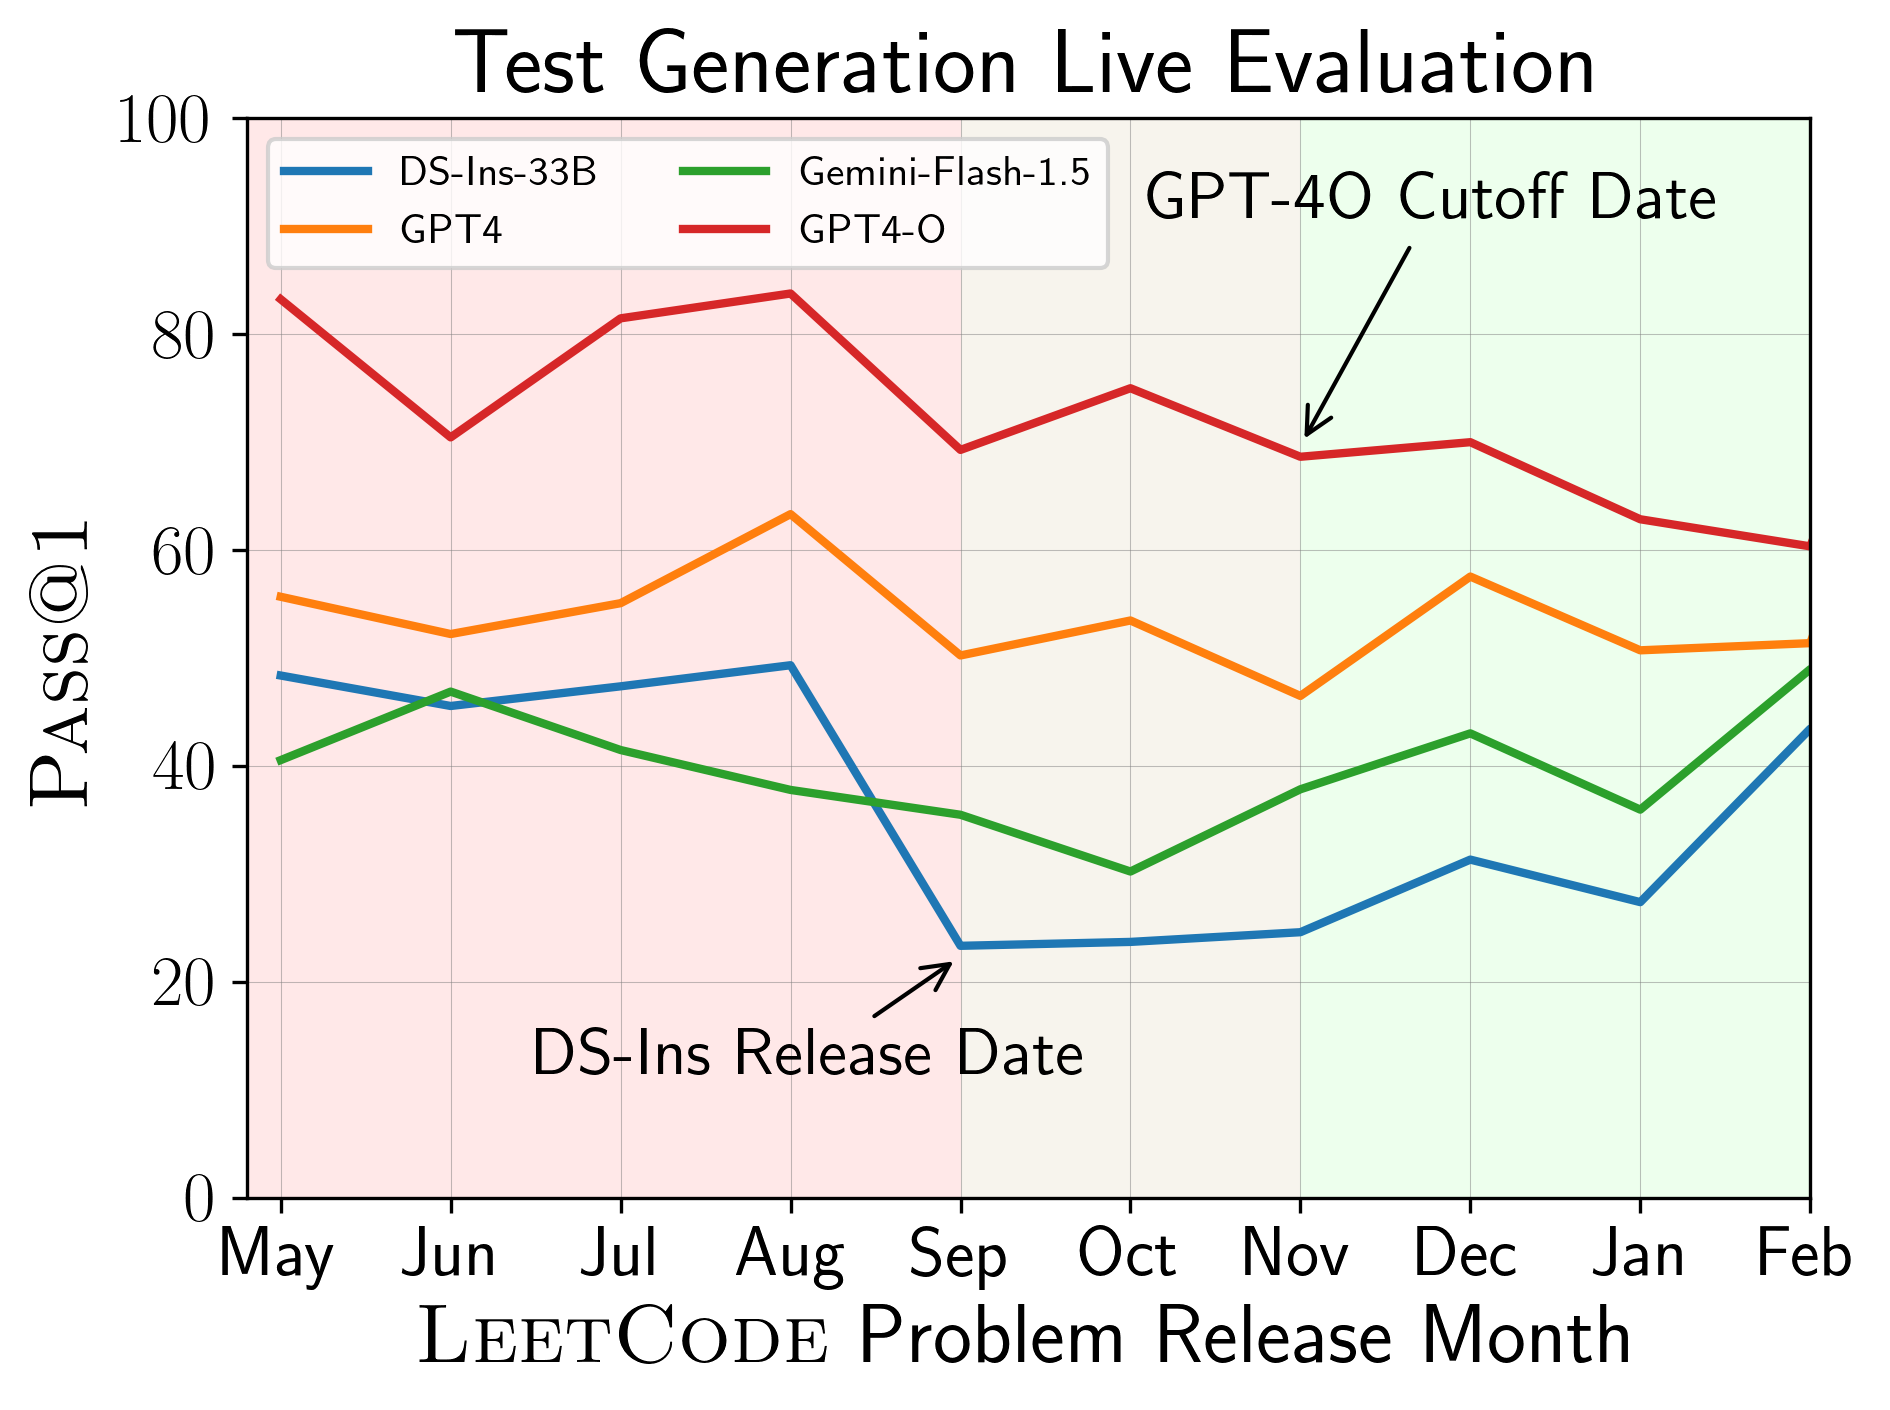
\includegraphics[width=0.49\linewidth]{figures/contamination_new/main_14_testgen_leetcode.png}
    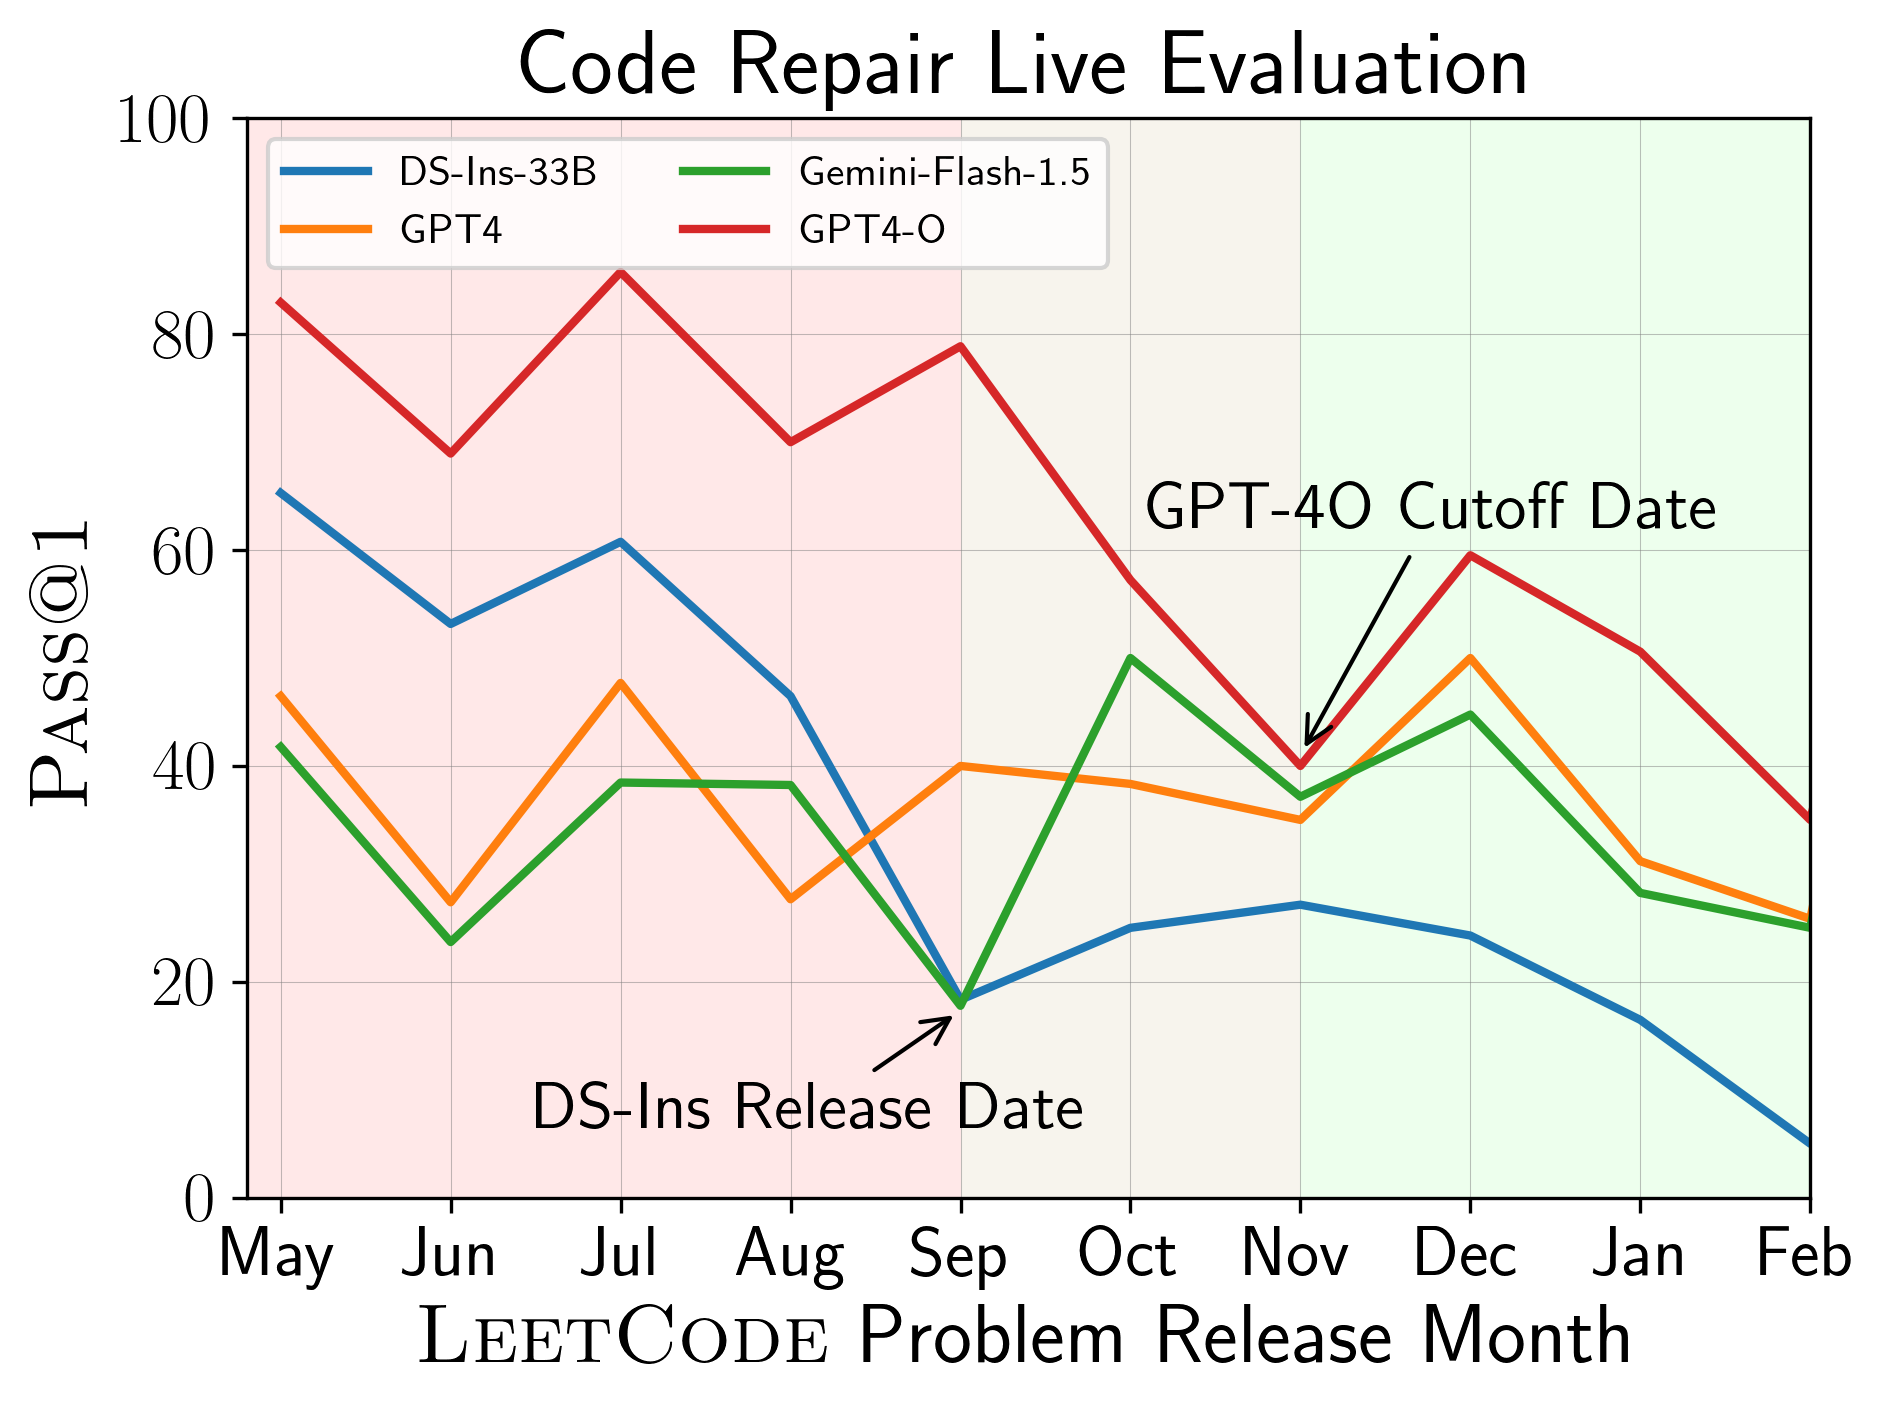
\includegraphics[width=0.49\linewidth]{figures/contamination_new/main_14_repair_leetcode.png}
    \hfil
    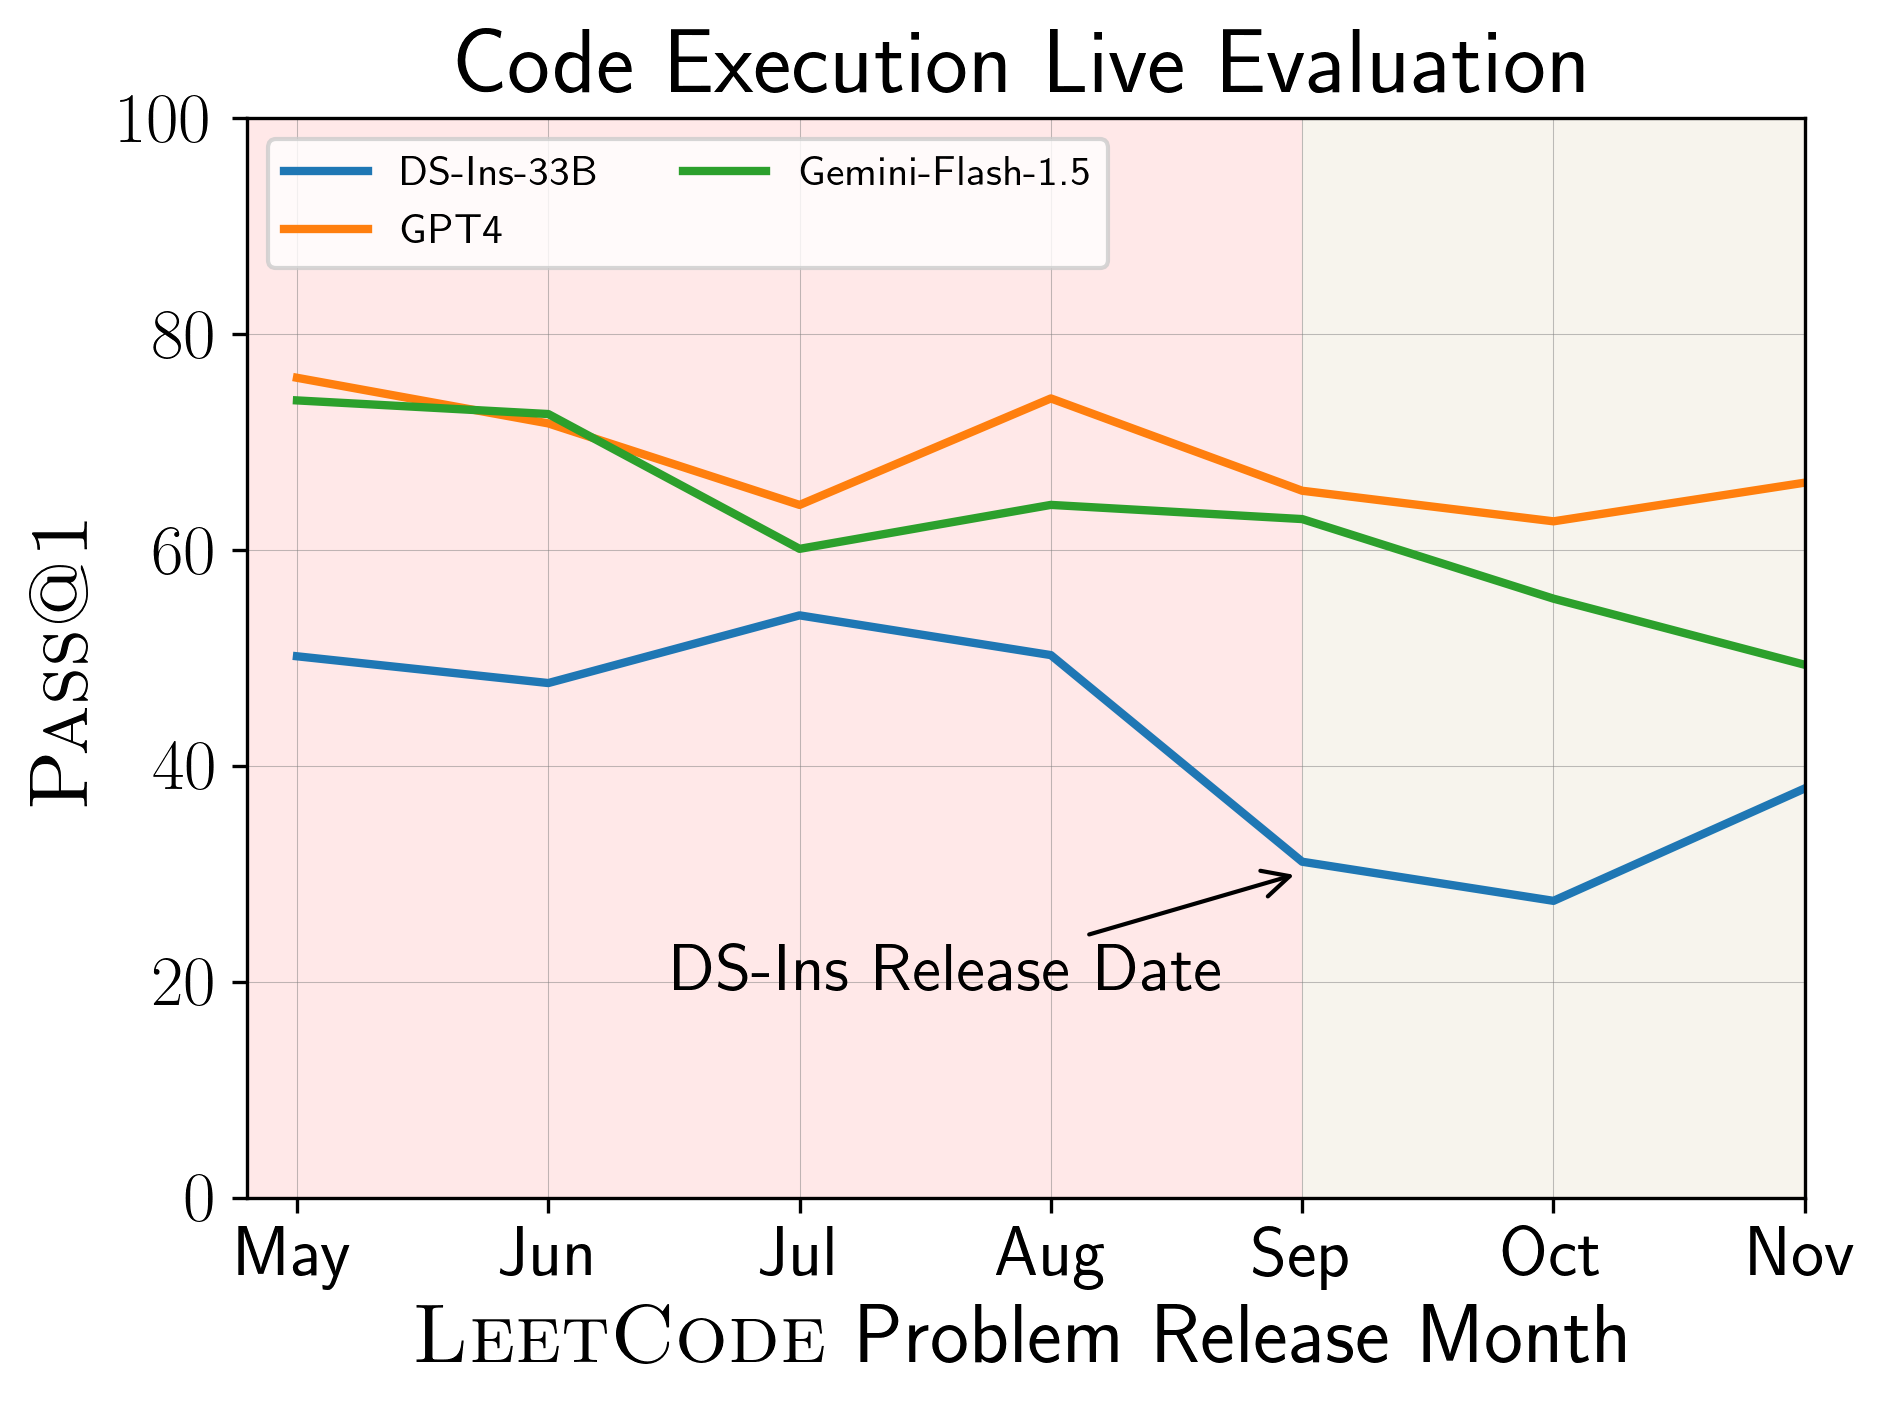
\includegraphics[width=0.49\linewidth]{figures/contamination_new/main_14_codeexec_leetcode.png}
    \caption{Contamination across code generation,
    test-output prediction, self-repair, and code execution scenarios over time.}
    \label{fig:lcb-contamination-all-tasks-thesis}
\end{figure}


\begin{figure}[H]
    \centering
    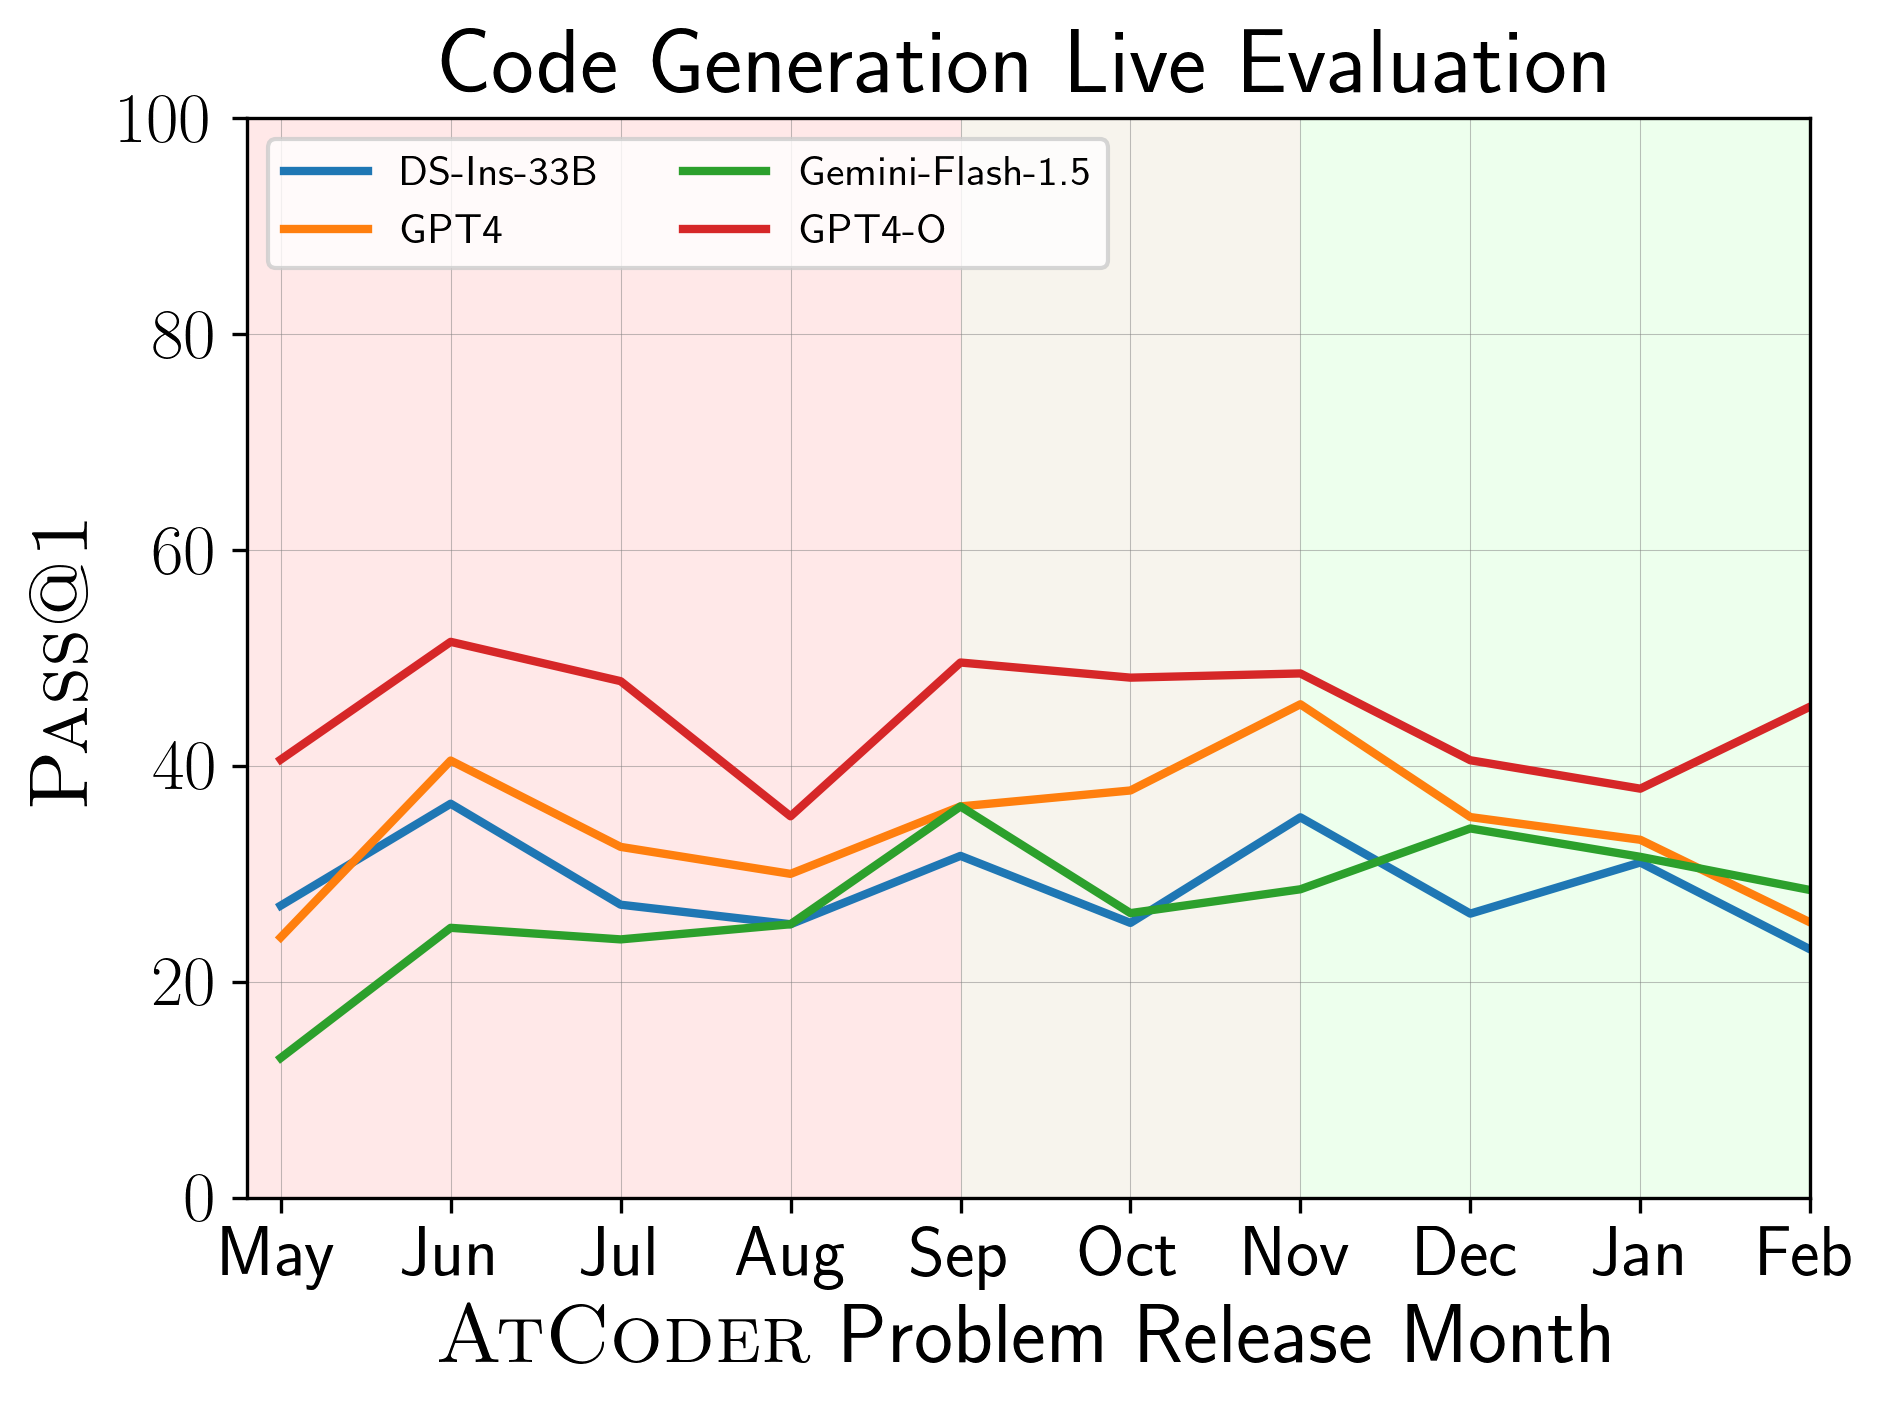
\includegraphics[width=0.55\linewidth]{figures/contamination_new/main_14_codegen_atcoder.png}
    \caption{Performance on problems released over different months for \atcoder{}.}
    \label{fig:lcb-atcoder-contamination-thesis}
\end{figure}

\noindent \textbf{Contamination Effects of Other Models:} In Figure~\ref{fig:lcb-contamination-all-models-thesis}, we show 
the performance of six models for each month between May $2023$ and Aug $2024$. \gptfourturbo{}, \mistrallarge{}, and \claudethrees{} were released in November $2023$, February $2024$, and March $2024$, respectively.
For these three models, we do not observe significant performance variations across months.
On the other hand, we observe that \deepseekbaseB{33} drops from \passmetric{1} $\smallsim 60$ in May problems to \passmetric{1} $\smallsim 0$ in September \leetcode{} problems,
suggesting significant contamination. Finally, \codestral{} achieves \passmetric{1} $36.5$ on problems released between May'23 and Jan'24 and \passmetric{1} $28.3$ on problems post Jan'24.

\begin{figure}[H]
    \centering
    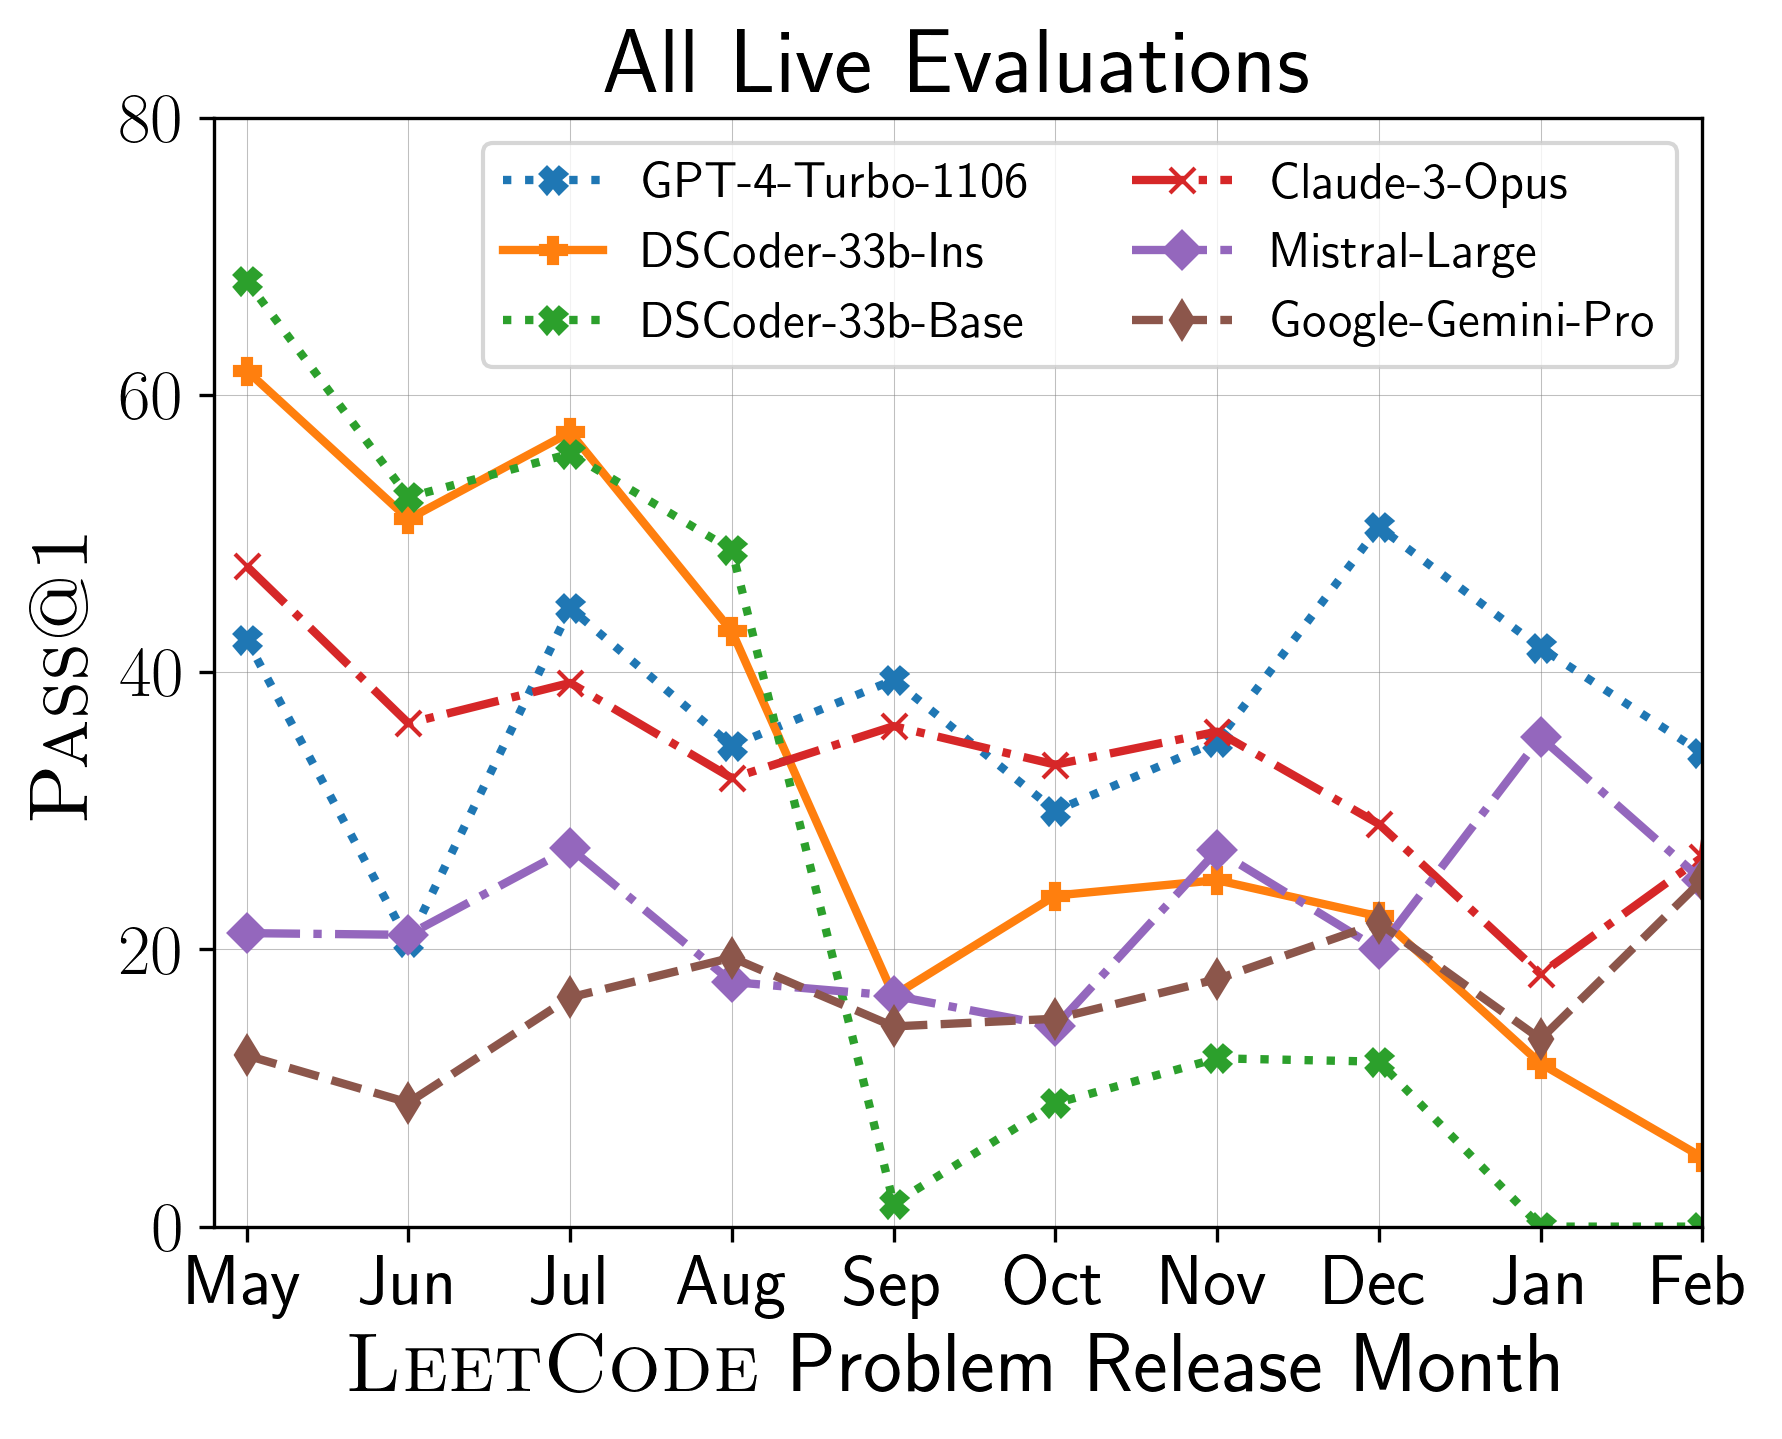
\includegraphics[width=0.49\linewidth]{figures/appendix/live_eval_custom_leetcode.png}
    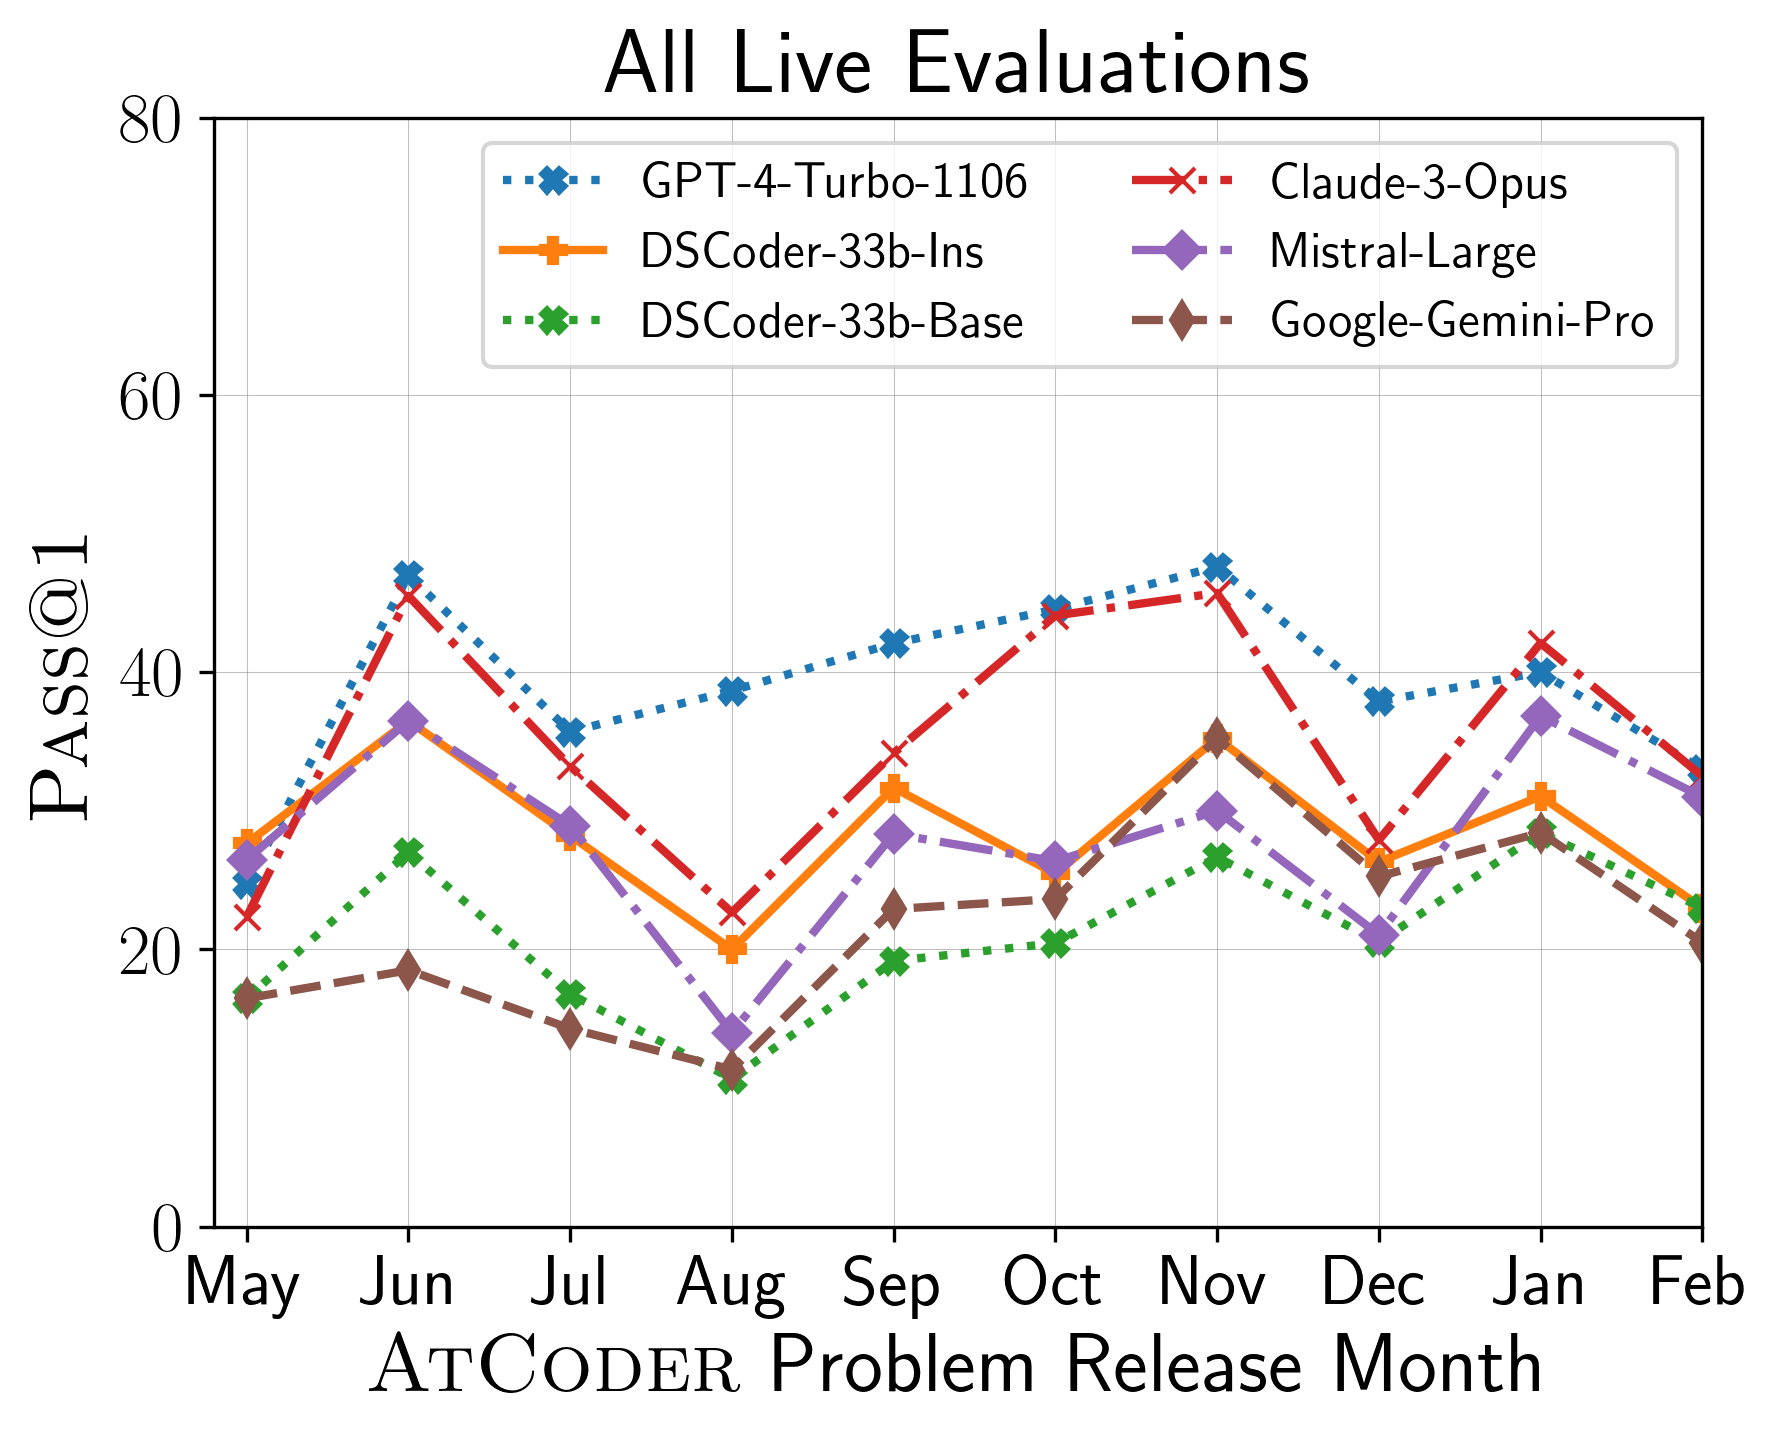
\includegraphics[width=0.49\linewidth]{figures/appendix/live_eval_custom_atcoder.png}
    \caption{Live evaluation over time for various models on code generation in
    \livecodebench{}.}
    \label{fig:lcb-contamination-all-models-thesis}
\end{figure}

\subsection{Holistic Evaluation}
\livecodebench{} also evaluates a broader set of coding capabilities. Instead of measuring 
only code generation, it evaluates four scenarios: code generation,
self-repair with execution feedback, code execution, and test-output
prediction. These scenarios are intended to isolate capabilities that appear in
real world software engineering workflows.

The four tasks, shown in \Cref{fig:holistic_tasks}, are as follows:

\begin{itemize}

\item \textbf{Code Generation:}
This is the standard setup used in previous benchmarks like HumanEval, MBPP, and APPS.
The model is given a problem statement consisting of a
natural language description and example tests (input-output pairs).
The task is to generate a correct solution passing all the tests.

\item \textbf{Self Repair:}
The self-repair scenario is based on previous works that tested the self-repair
capabilities of \llms{}~\citep{olausson2023demystifying,shinn2023reflexion,chen2023teaching}.
Here, the model is given a problem statement from which it generates a
candidate program. If the program is incorrect, the model is additionally provided with error
feedback, either the exception message or a failing test case, and is tasked
with generating the fixed solution. 

\item \textbf{Code Execution:}
The code execution scenario is based on the output prediction setup used in
\cruxeval{}~\citep{gu2024cruxeval}. The model is provided a program snippet
consisting of a function (\texttt{f}) along with a test input to the program
and is tasked with predicting the output of the program on the input test case.

\item \textbf{Test Case Output Prediction:}
The test case output prediction task is designed to study natural
language reasoning and test generation. In this task, the model is given the
problem statement along with a test input, and it is asked to generate the
expected output of that input.

\end{itemize}

\begin{figure}[H]
    \centering
    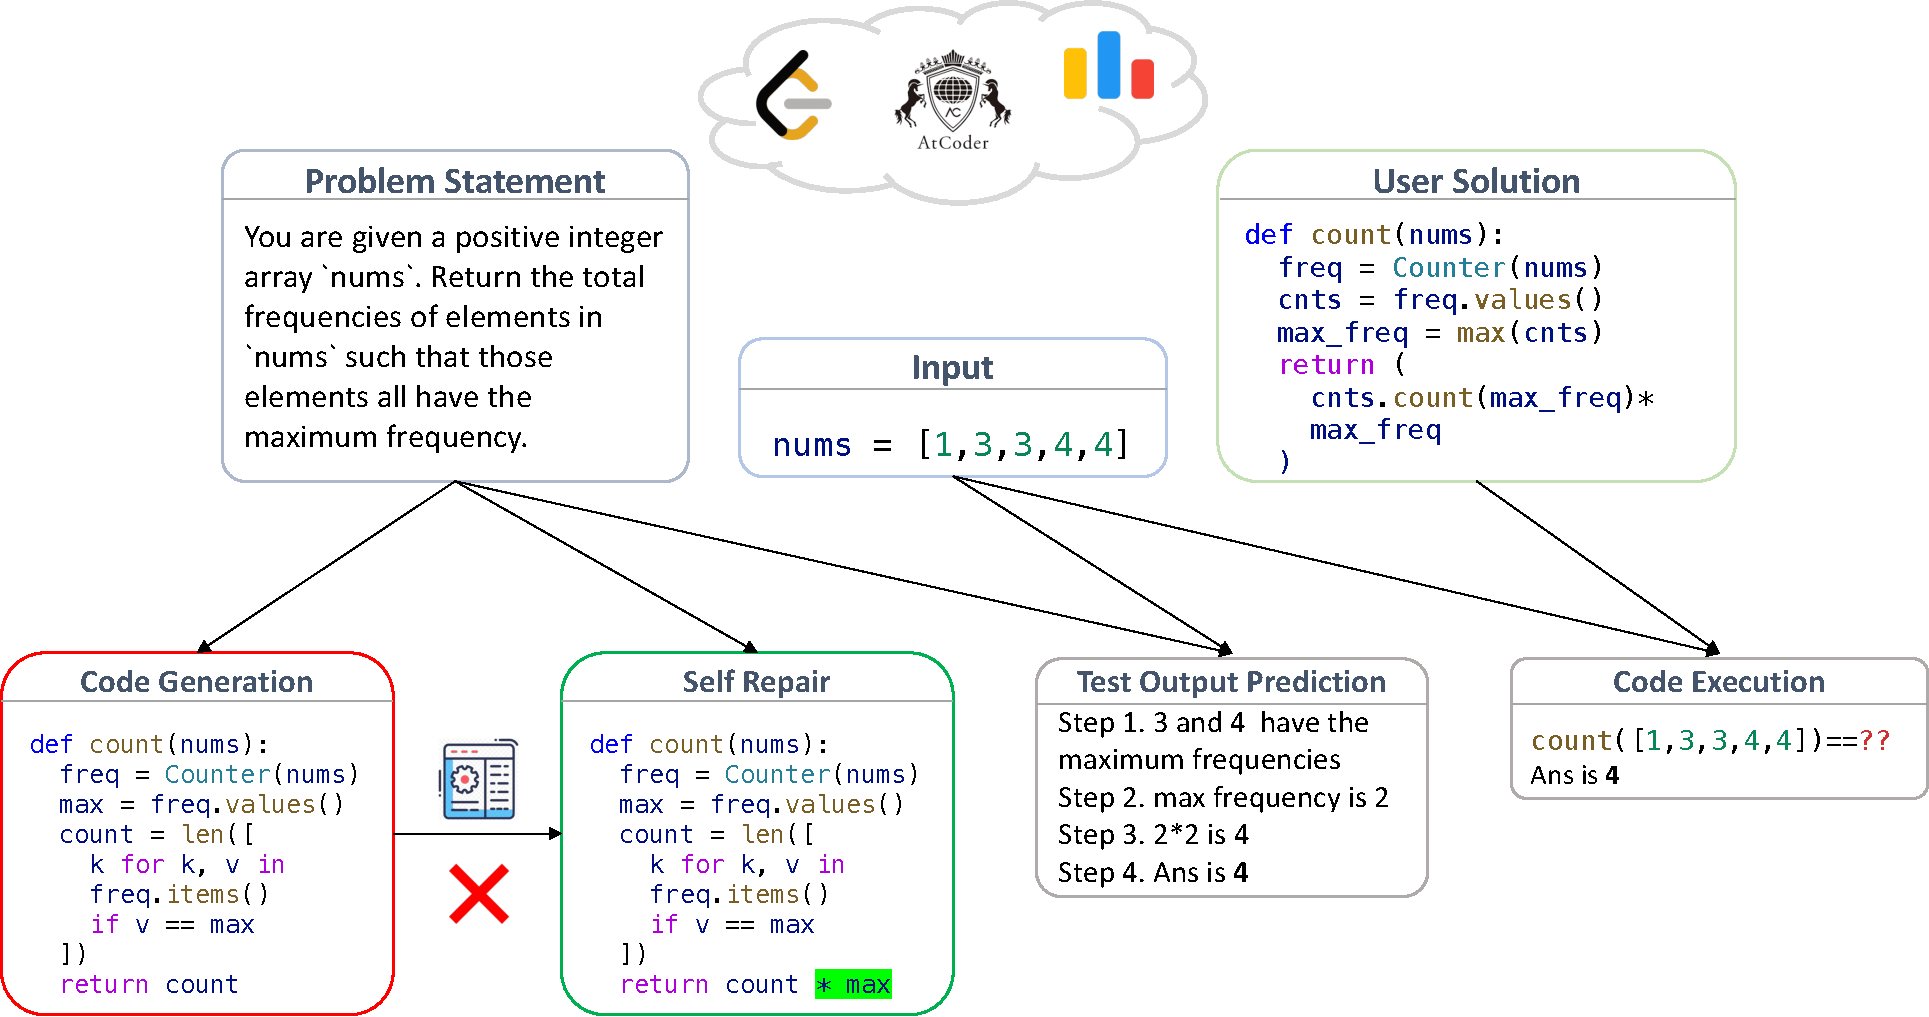
\includegraphics[width=0.85\textwidth]{figures/overview/LCB_holistic_tasks.pdf}
    \caption{
        Overview of the four scenarios present in \livecodebench{}.
        %Coding is multi-faceted and we propose evaluating \llms{} on a suite of evaluation setups that capture various coding-related capabilities.
        %Specifically, beyond the standard code generation setting, we consider three additional scenarios, namely self-repair, code execution, and a newly introduced test output prediction task.
        }
    \label{fig:holistic_tasks}
    \vspace{-15pt}
\end{figure}

In \Cref{fig:all_tasks_radial}, we show a high-level view of how various models perform
across the four scenarios. We observe that relative model differences change across
code generation, self-repair, code execution, and test-output prediction. 

\begin{figure}[H]
    \centering
    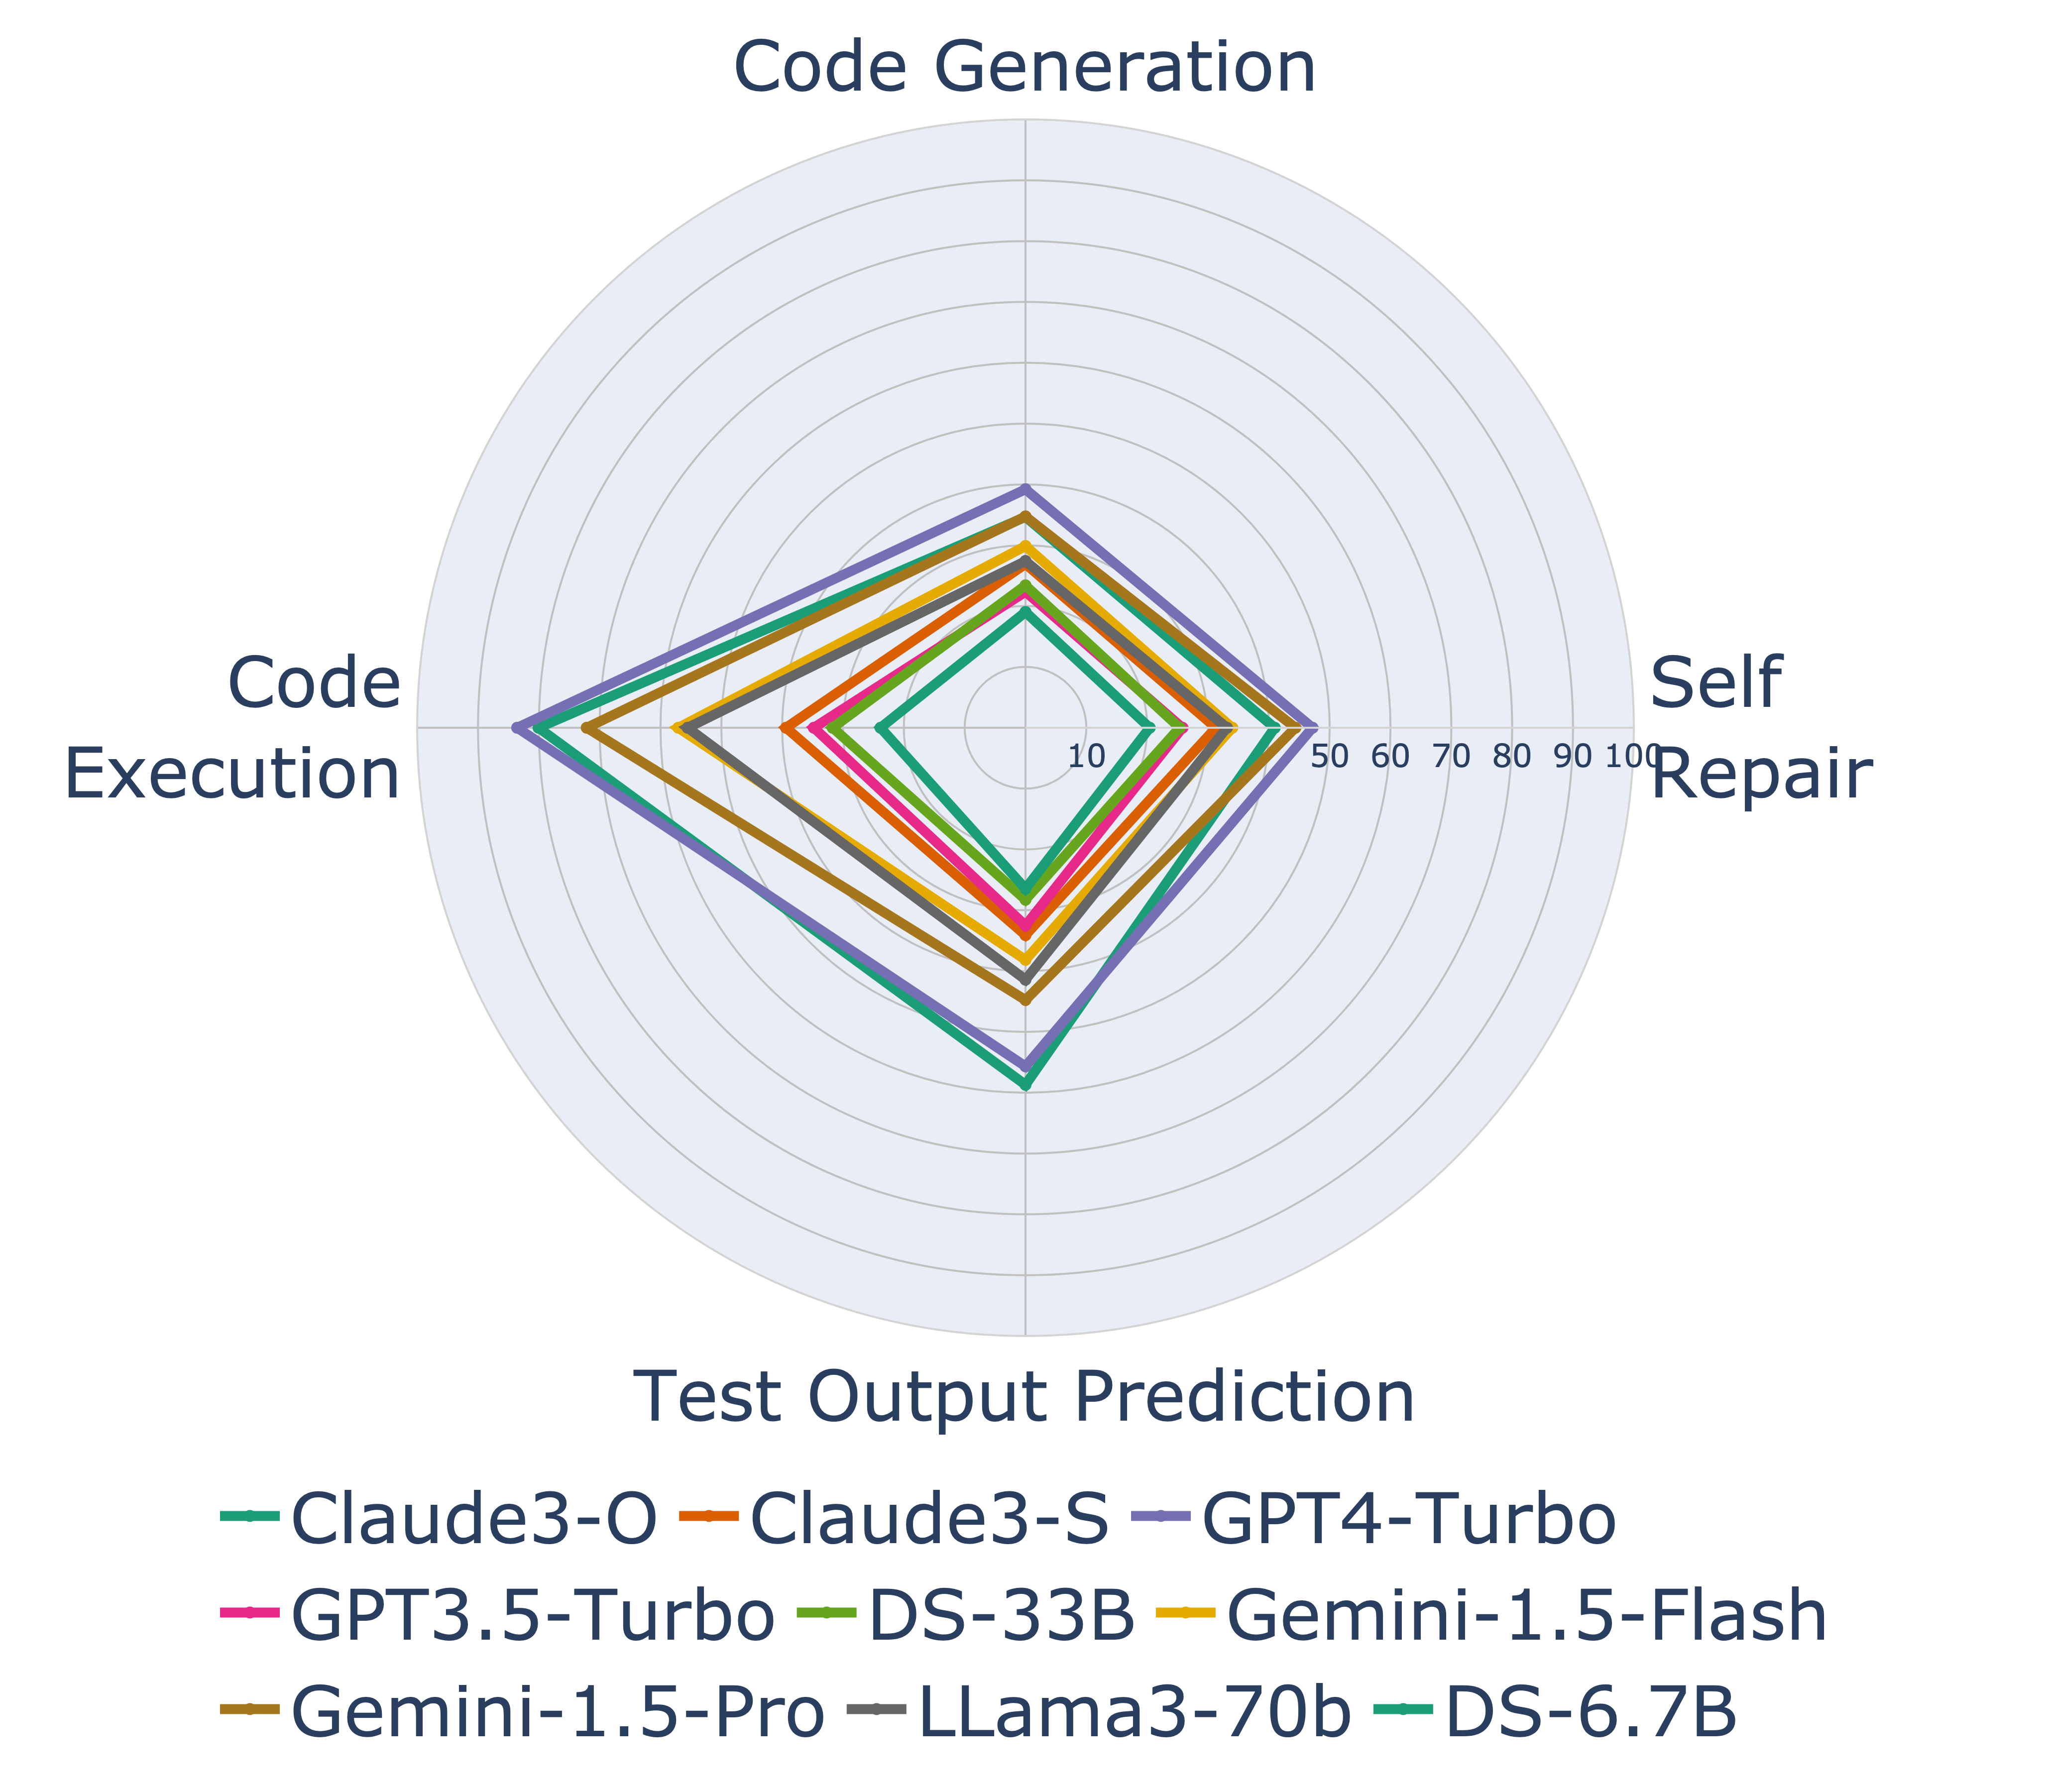
\includegraphics[width=0.72\linewidth]{figures/overview/tasks_radar.png}
    \caption{Scenario-level performance profiles in \livecodebench{}.}
    \label{fig:all_tasks_radial}
\end{figure}


Next, in \Cref{fig:results_plots}, we show the full results of all models across each scenario.
This reveals that relative model performance is related across scenarios, with high correlations between
\passmetric{1} scores. However, there are changes in relative gaps. After self-repair, \gptfourturbo{} increases its lead over \gptfour{}.
\claudeopus{} and \mistrallarge{} perform well on the more reasoning and CoT-based scenarios, code execution and
test-output prediction. 

\begin{figure}[H]
  \centering
  \begin{minipage}[t]{0.49\textwidth}
    \centering
    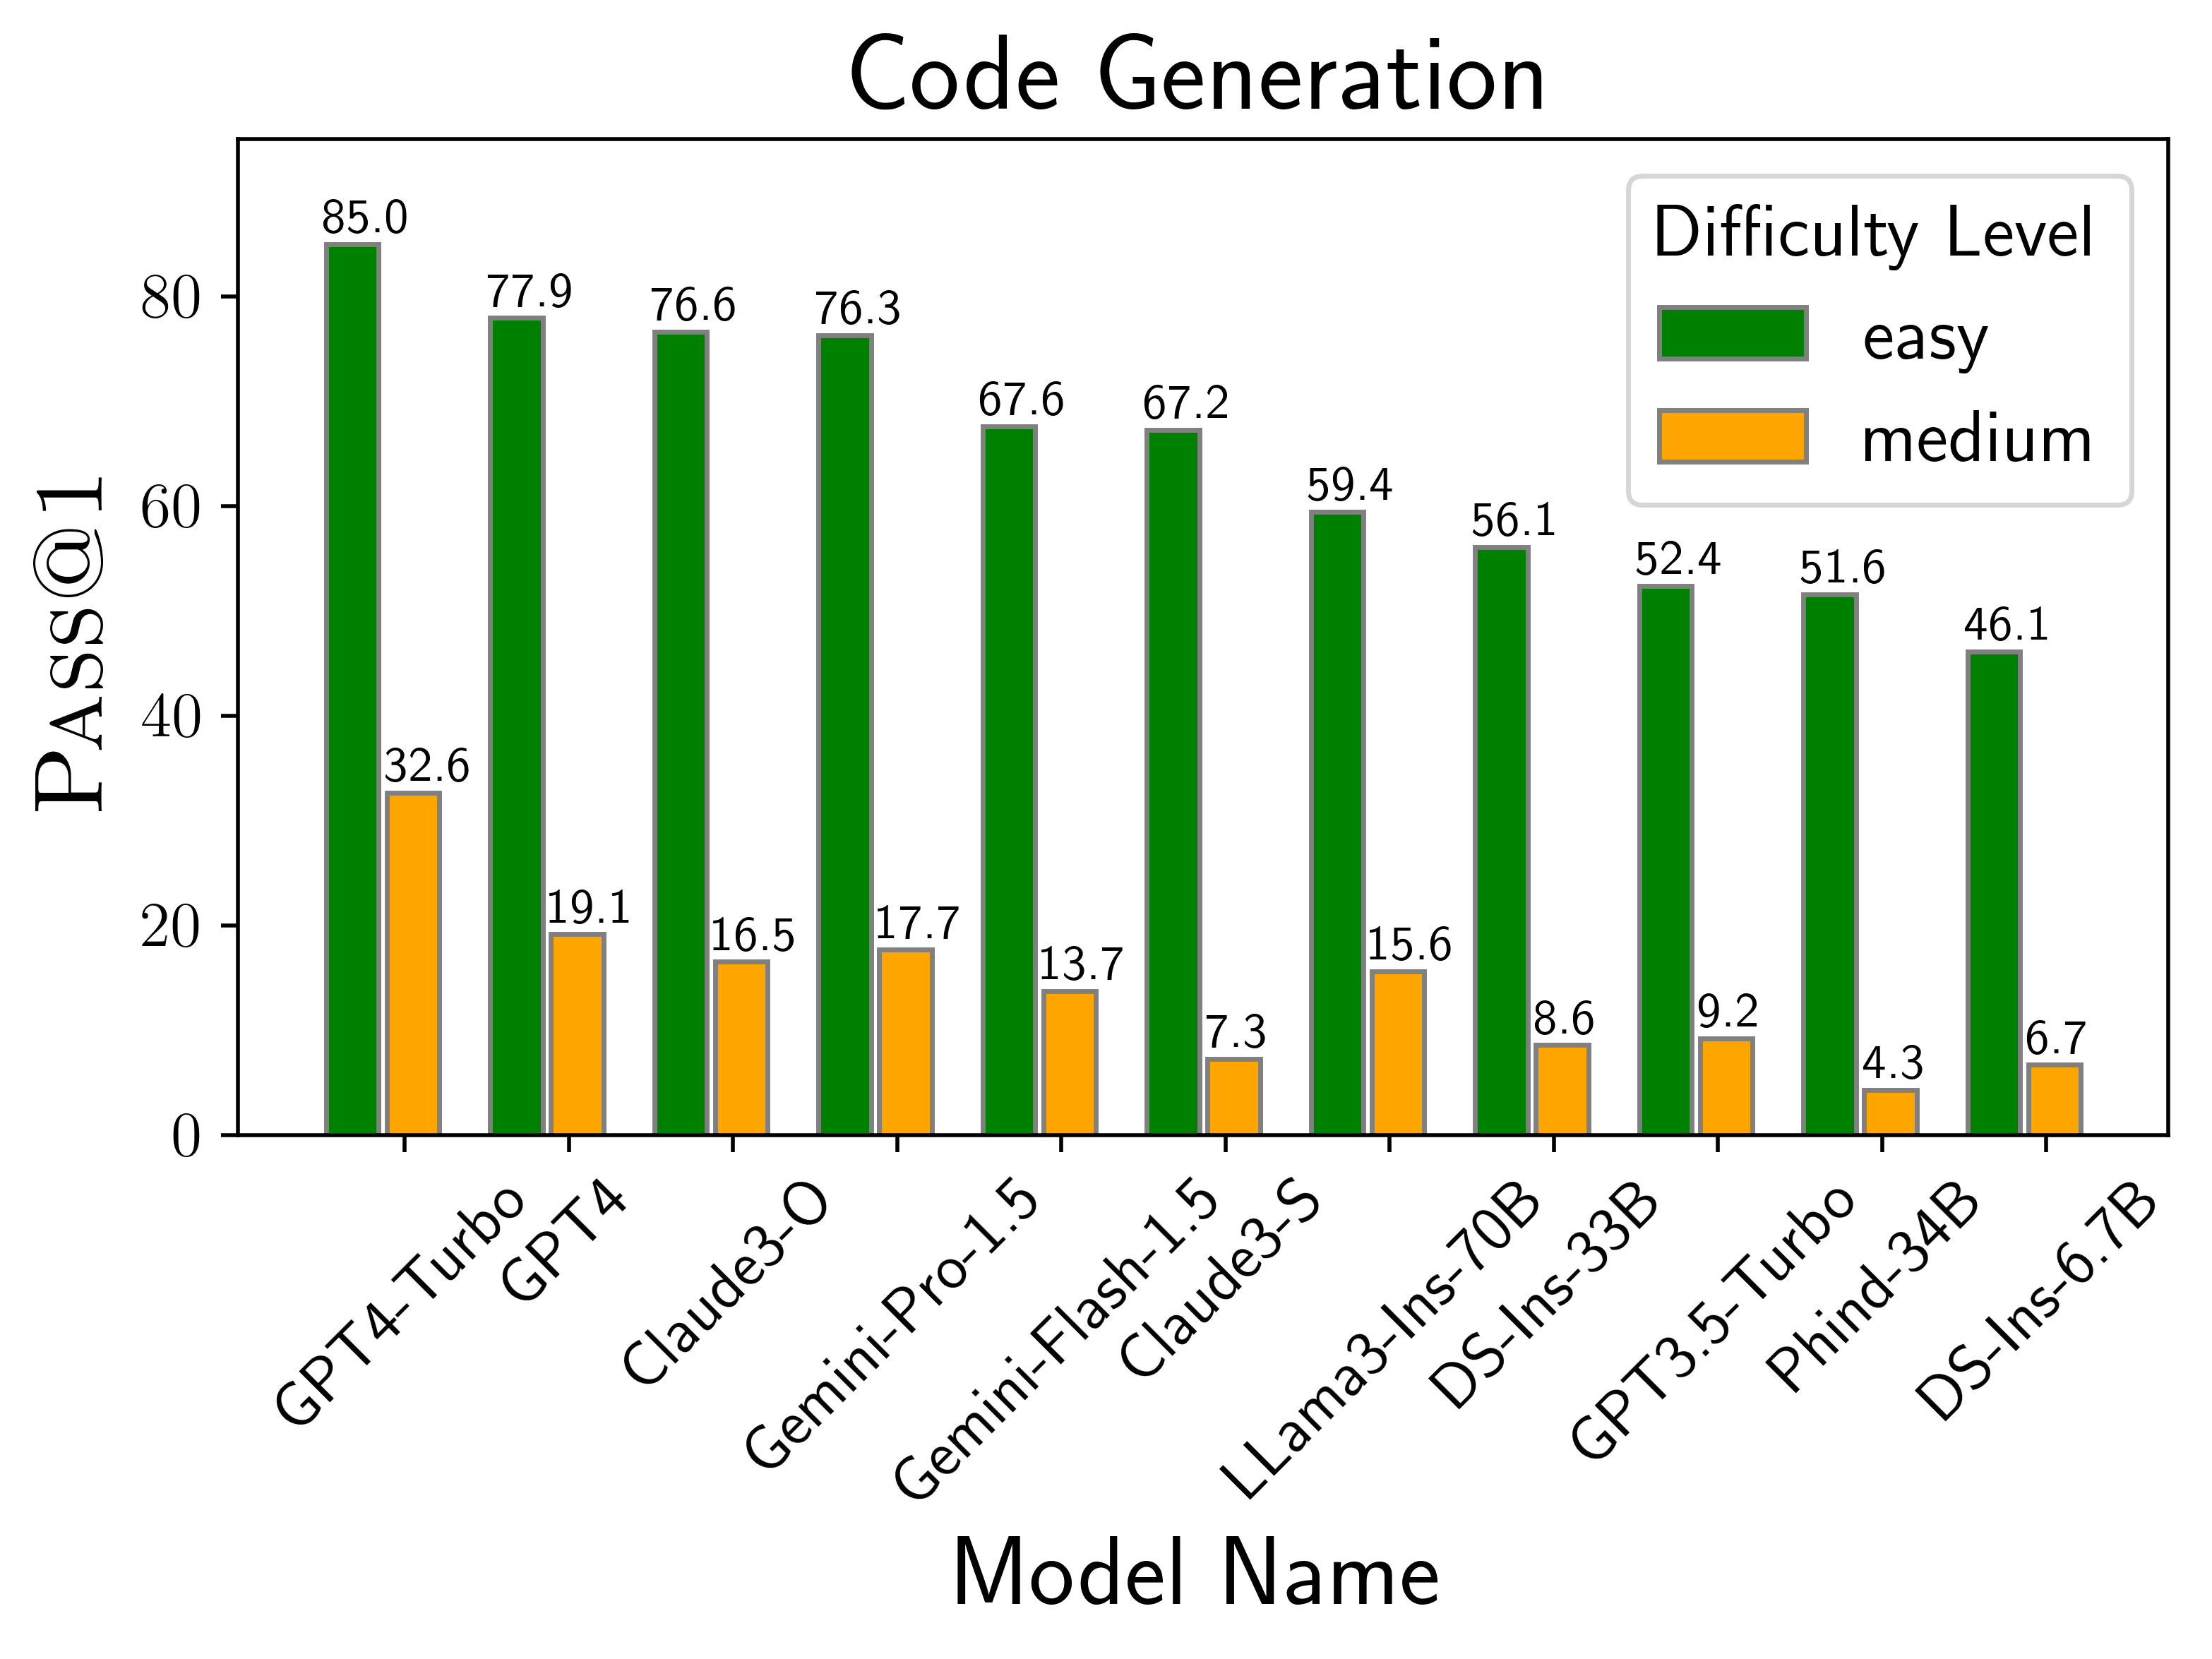
\includegraphics[width=\linewidth]{figures/main_results/codegen_performance.png}
  \end{minipage}\hfill
  \begin{minipage}[t]{0.49\textwidth}
    \centering
    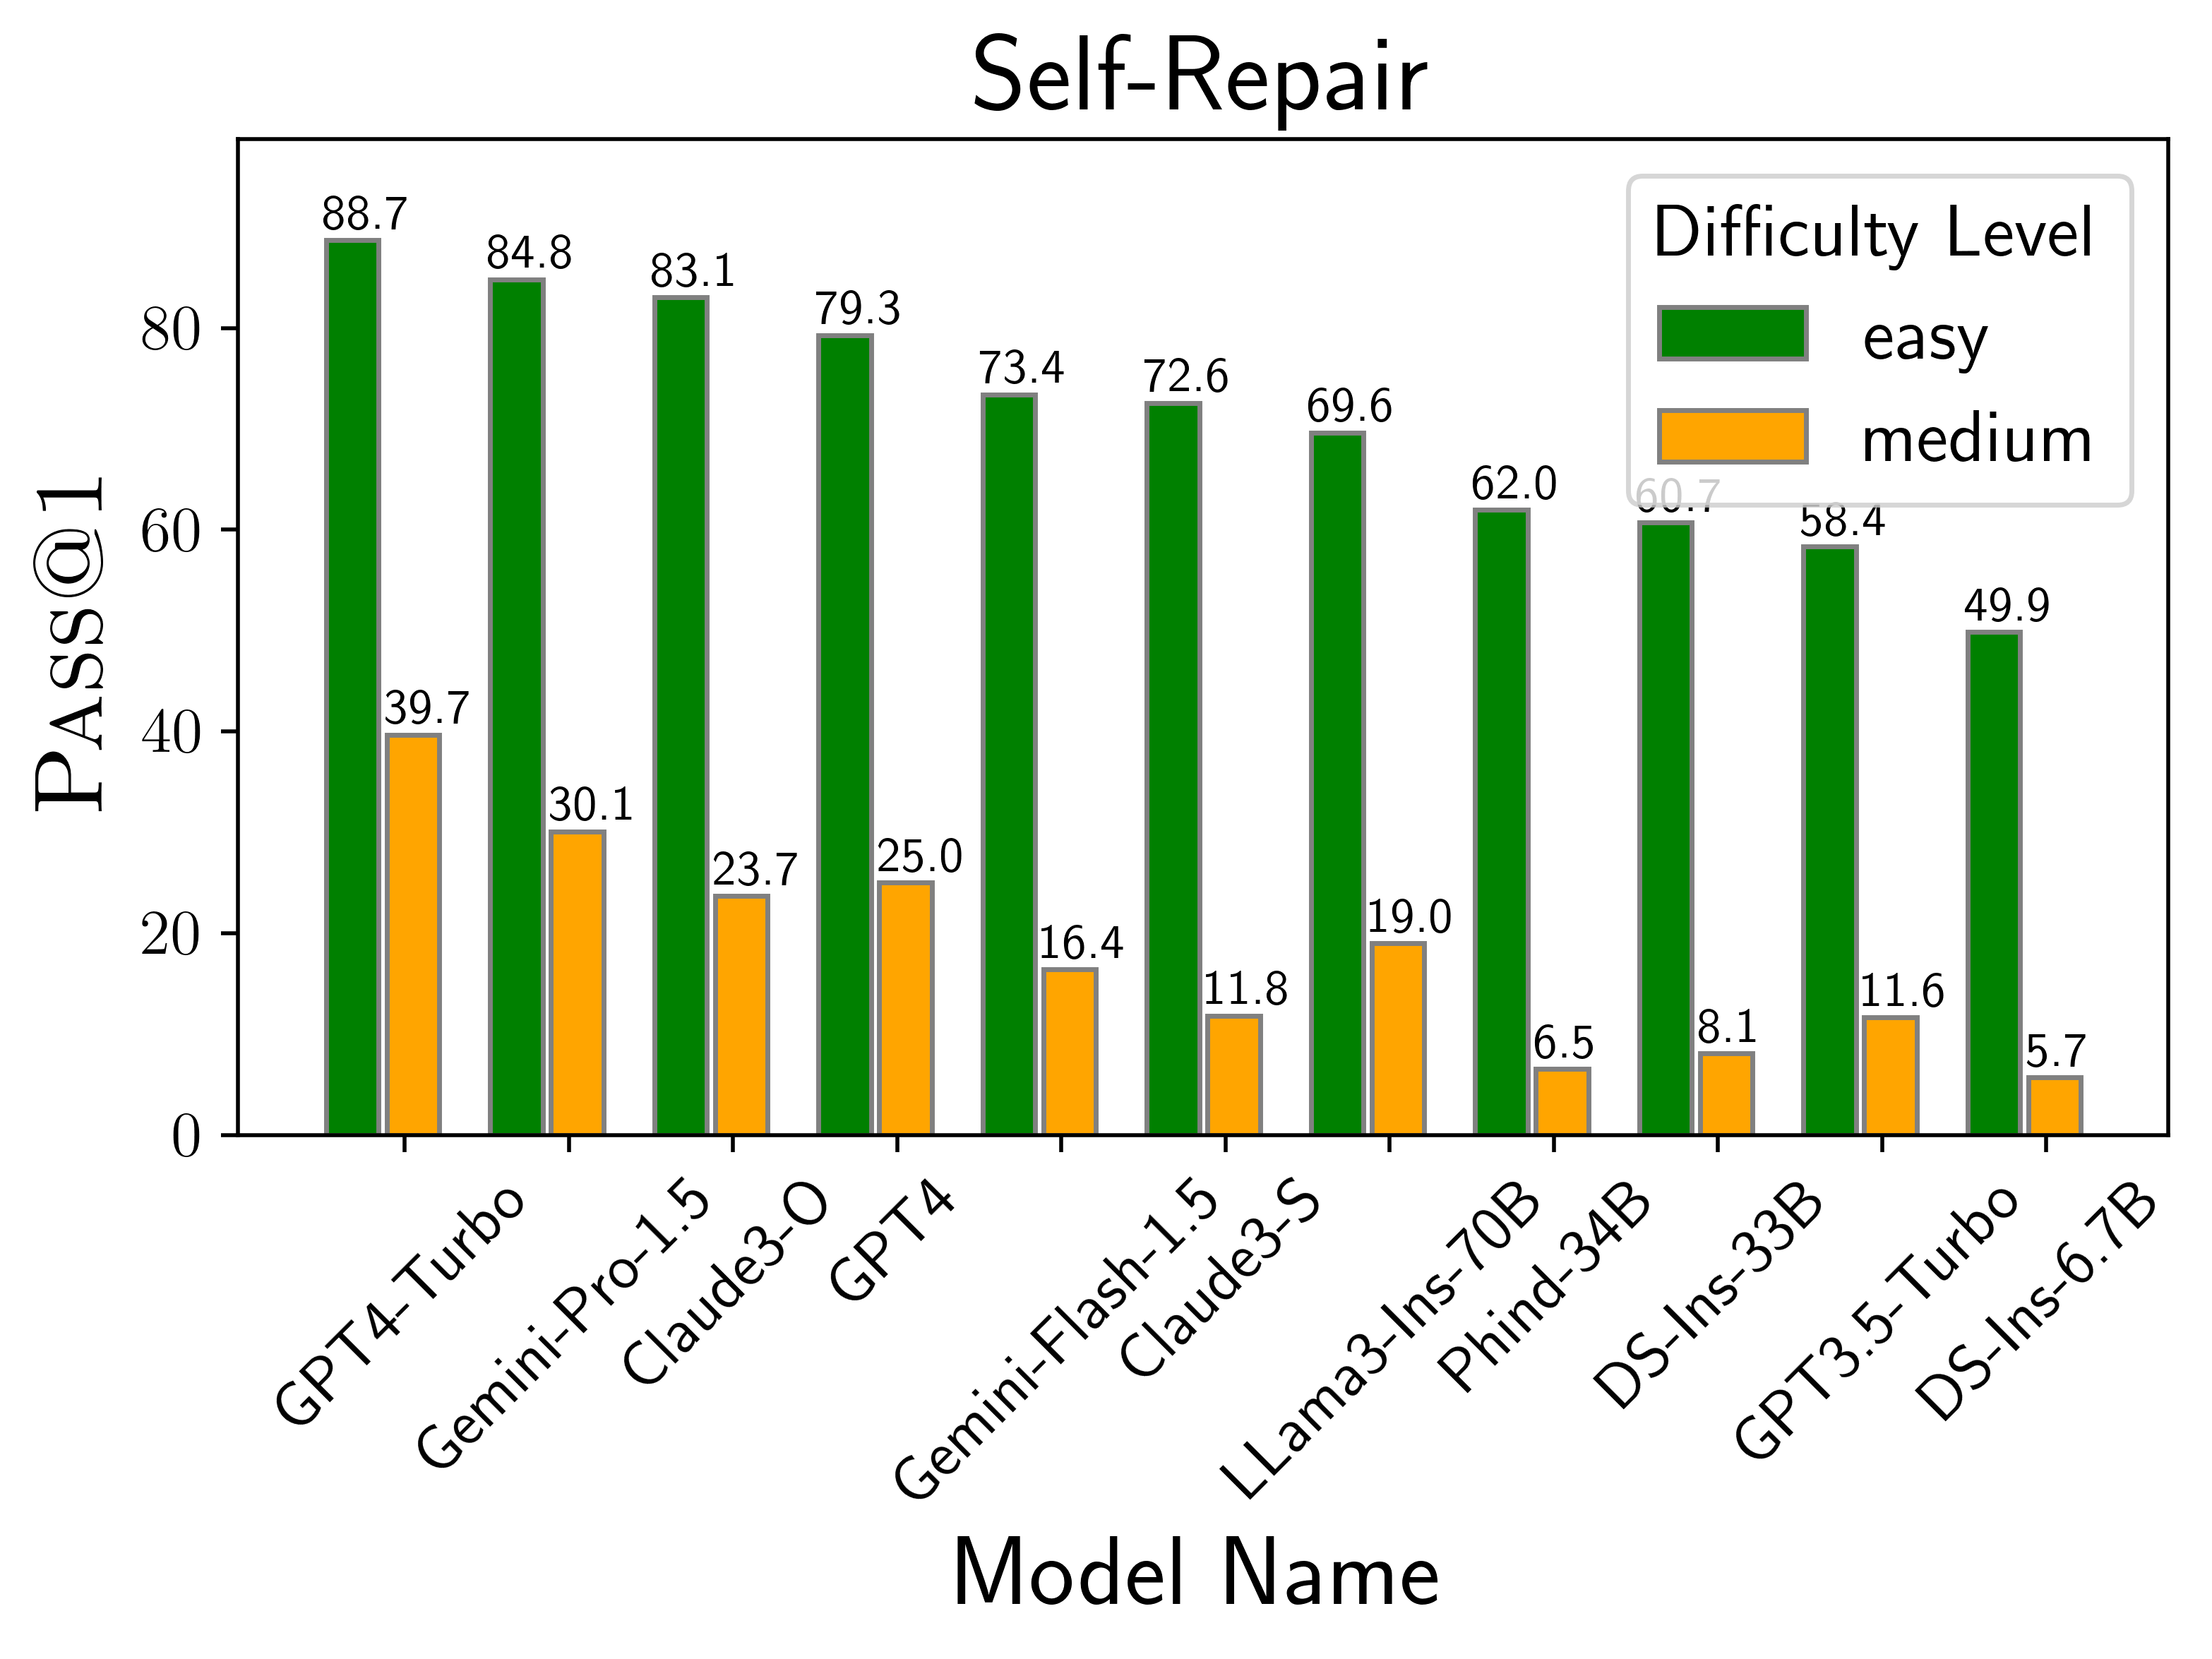
\includegraphics[width=\linewidth]{figures/main_results/repair_performance.png}
  \end{minipage}

  \vspace{0.5em}

  \begin{minipage}[t]{0.49\textwidth}
    \centering
    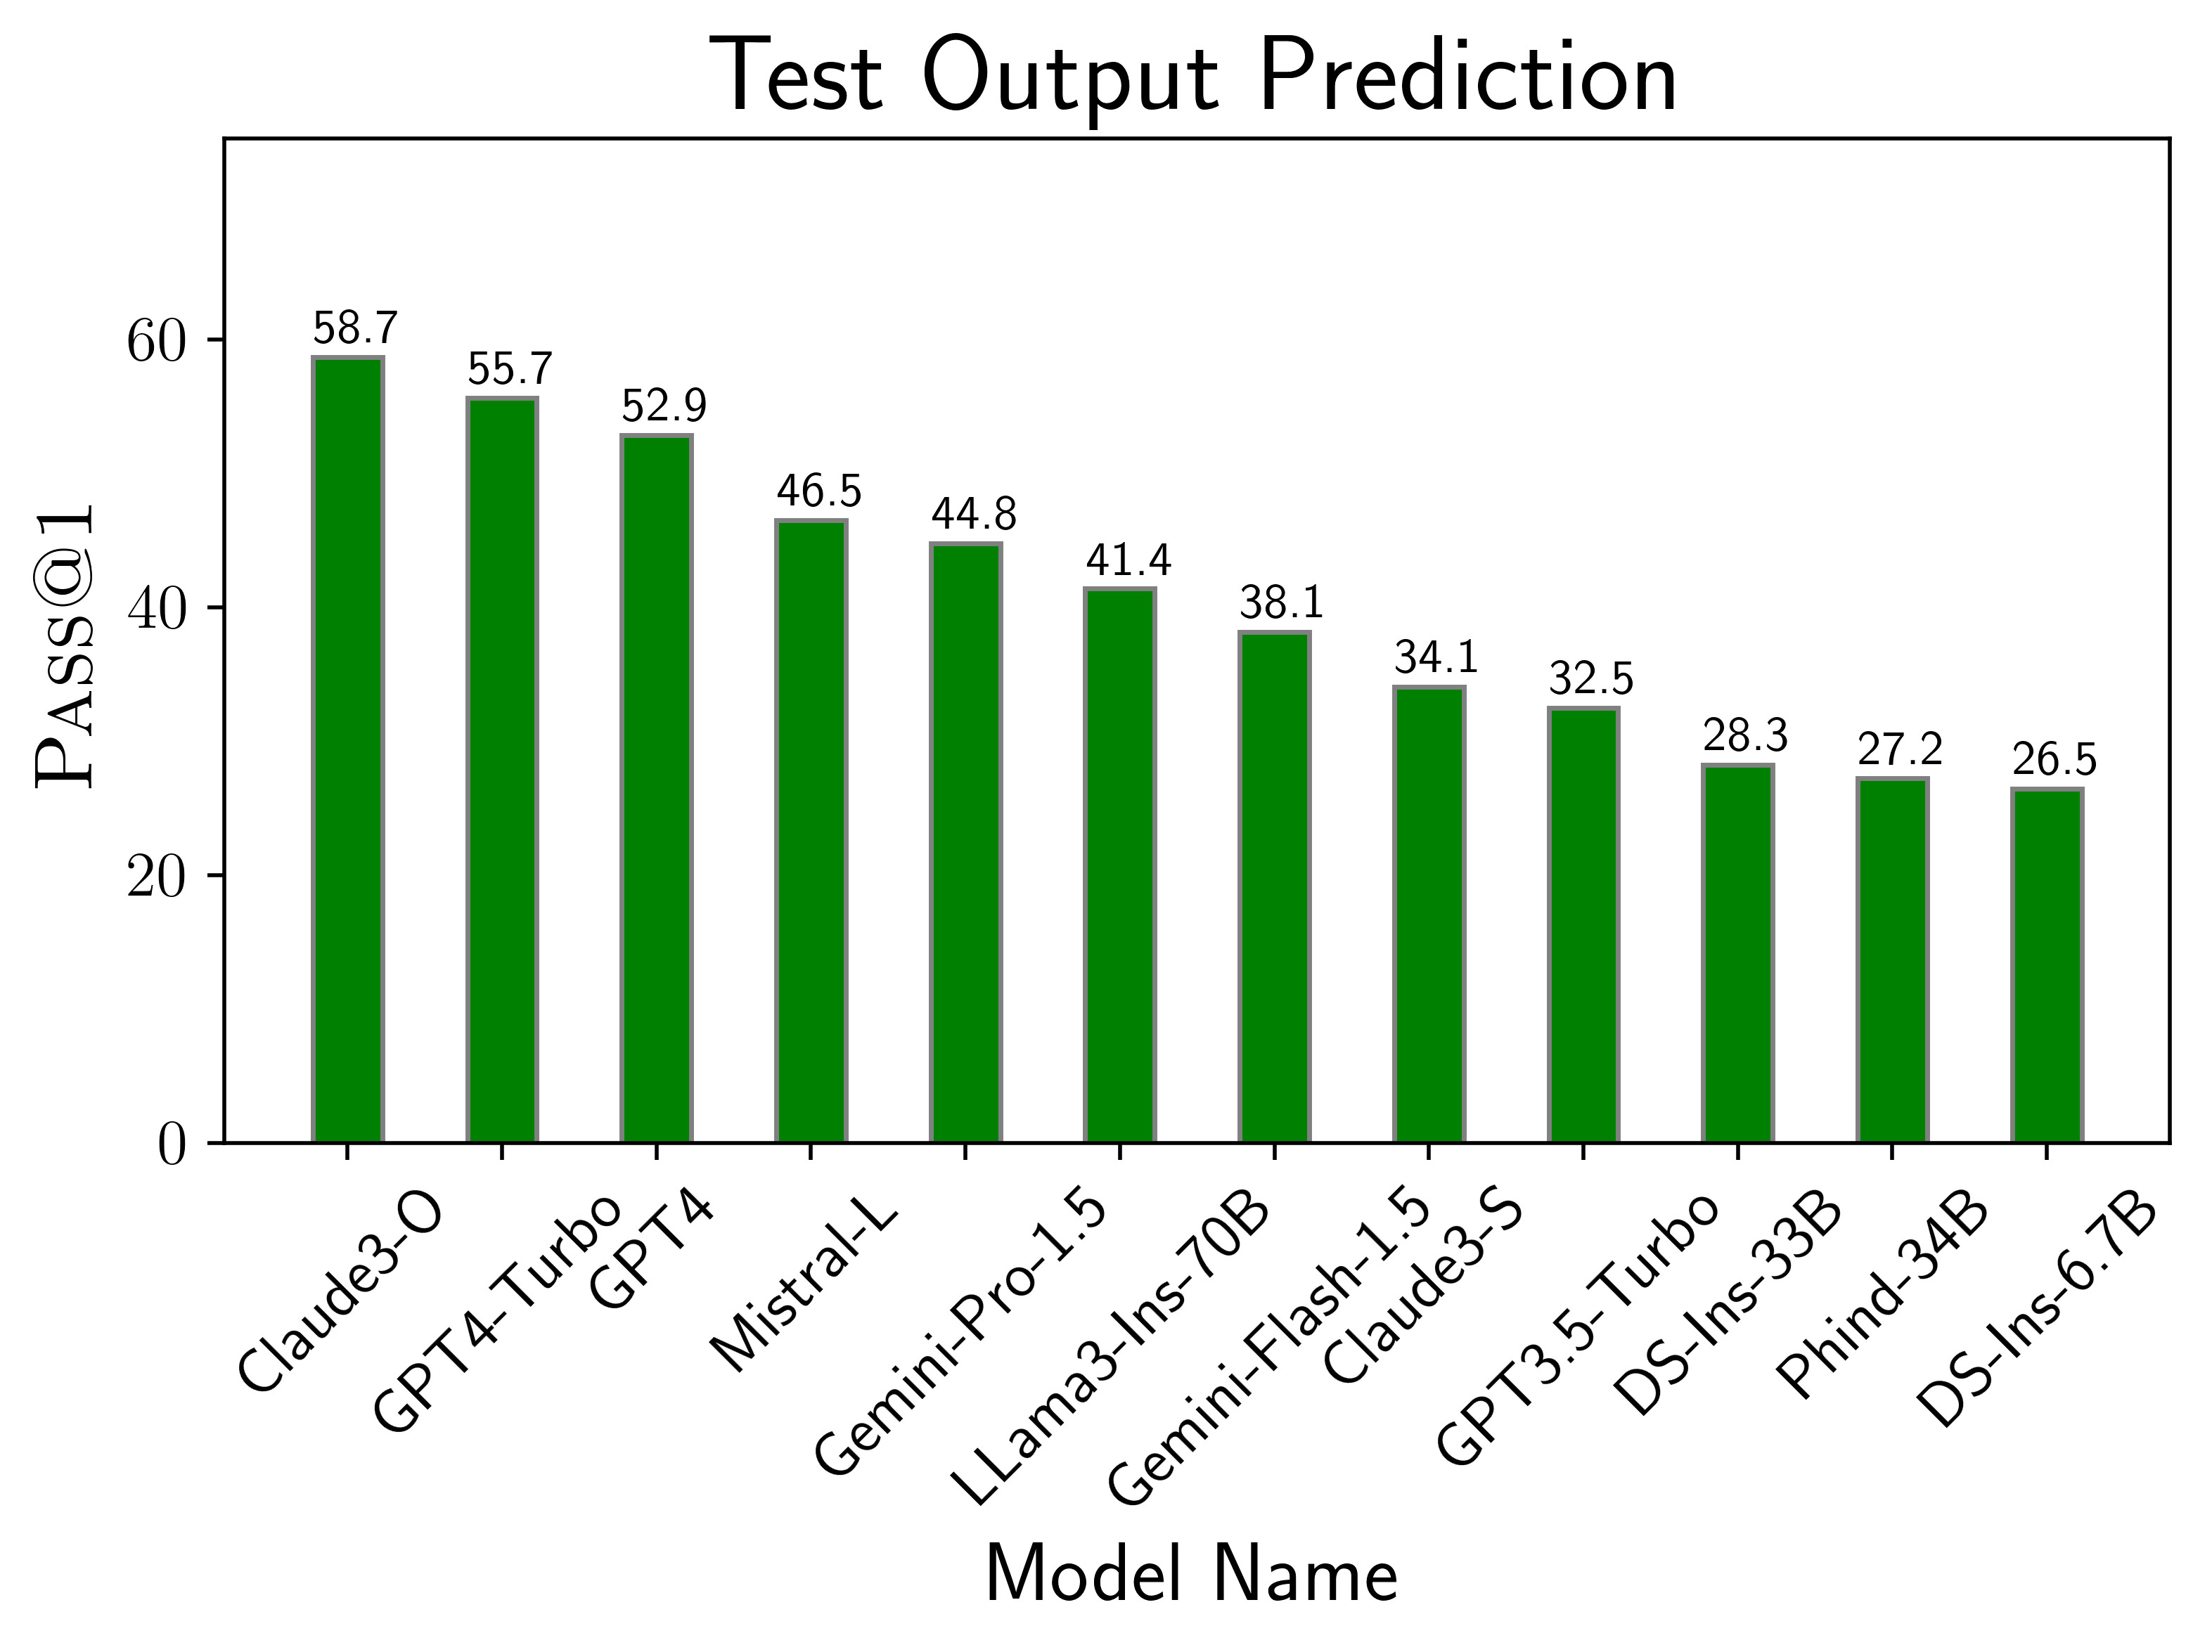
\includegraphics[width=\linewidth]{figures/main_results/testgen_performance.png}
  \end{minipage}\hfill
  \begin{minipage}[t]{0.49\textwidth}
    \centering
    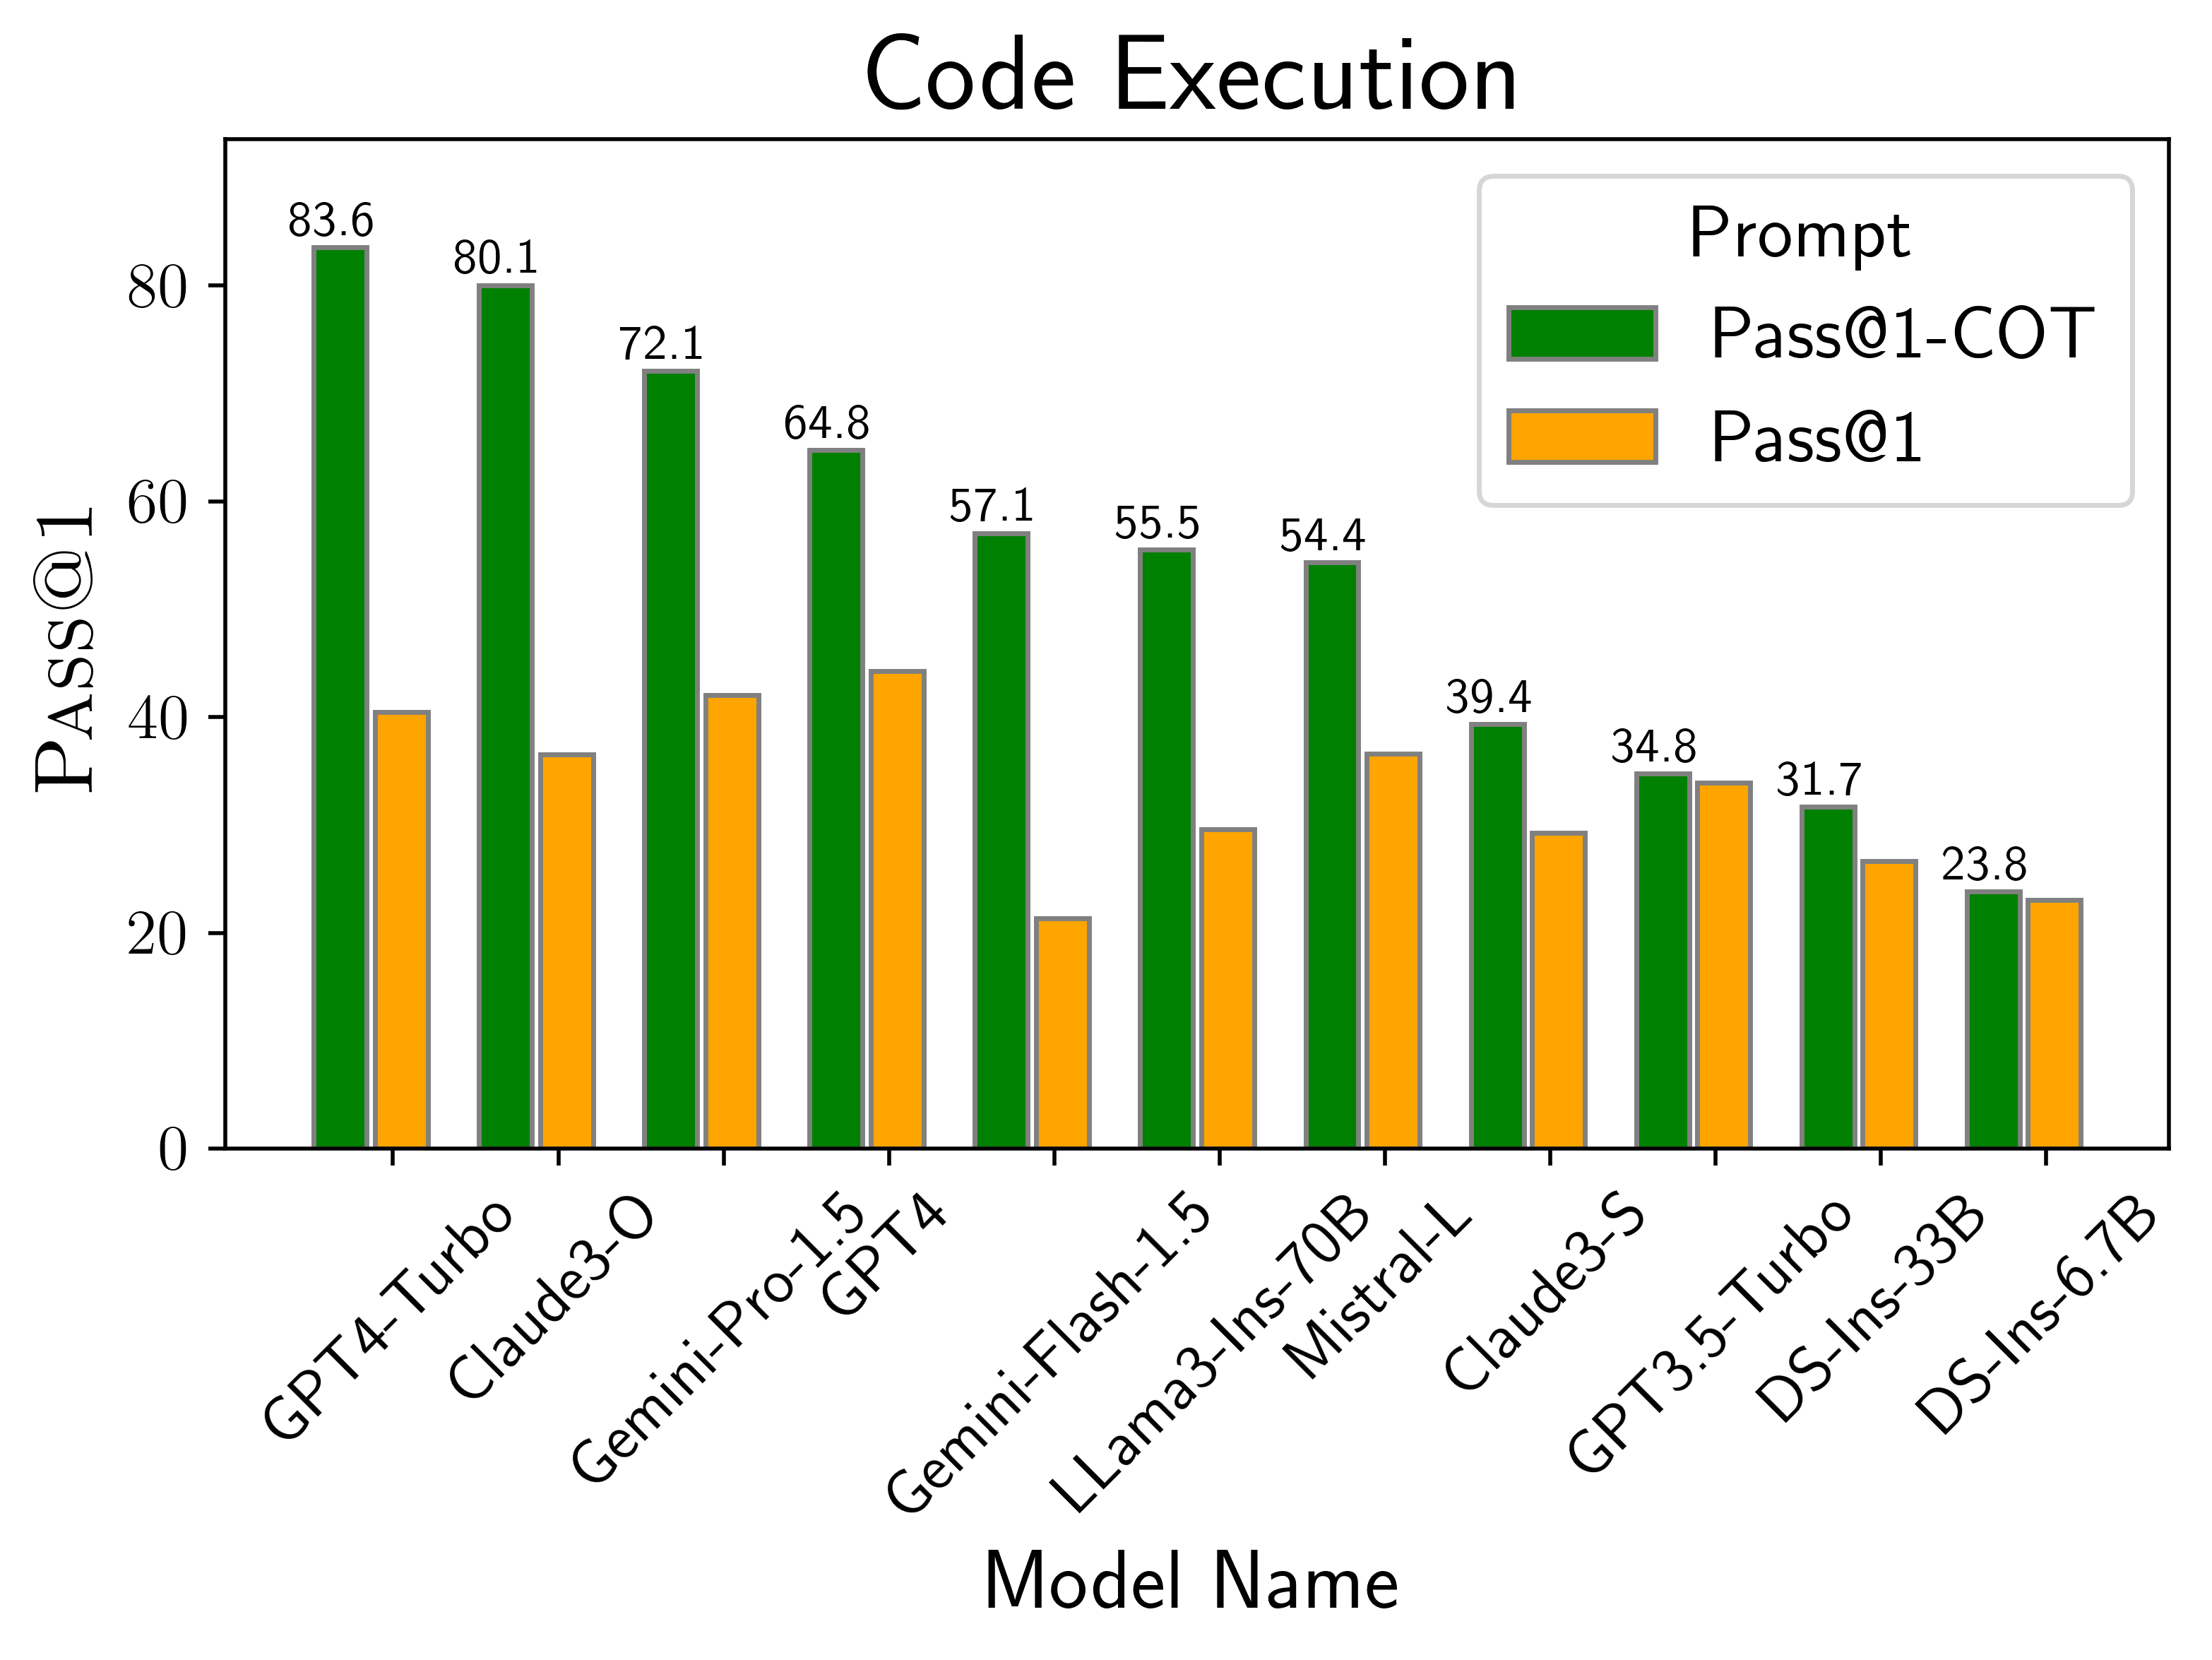
\includegraphics[width=\linewidth]{figures/main_results/execution_performance.png}
  \end{minipage}

  \caption{Model performances across the four scenarios available in \livecodebench{}.}
  \label{fig:results_plots}
\end{figure}
  


\subsection{Discussion}
In \livecodebench{}, we show how crucial it is to account for data contamination when 
evaluating code models. As we saw, model performance often drops sharply on problems
released after a model's training cutoff date. Failing to taking this bias into account will
lead to misleading comparisons between models, as one model may have seen problems that another model has not.
Through our holistic scenario design, we also saw that there are important differences in 
the ability of frontier language models to perform code generation, repair, execution, and 
test-output reasoning. Overall, \livecodebench{} provides a clearer and more holistic picture
of the algorithmic coding capabilities of language models while setting a standard for
future benchmarks to control for contamination biases. 
